% Project report. Reuses the paper's shared sections as chapters and adds
% report-only chapters from report/. Shared files use \sect/\subsect, which
% become \chapter/\section here.
% Build: latexmk -pdf report.tex
\documentclass[12pt,a4paper,oneside]{report}
% Packages and macros shared by every build (paper-ieee, paper-lncs, report).
% Each wrapper defines \sect, \subsect and the widefigure environment before \input-ing sections.
\usepackage[T1]{fontenc}
\usepackage[utf8]{inputenc}
\usepackage{amsmath,amssymb}
\usepackage{graphicx,booktabs,tabularx,array}
\usepackage{url,xurl}
\usepackage{xcolor}
\usepackage{microtype}
\setlength{\emergencystretch}{2em}
% Visible placeholder for text still to be written. Shows in red in the PDF.
% Build with \def\final{} before \documentclass... or just search for \todo before submitting.
\newcommand{\todo}[1]{\textcolor{red}{[TODO: #1]}}
% Full vs conference text. In sections/, write
%   \iffull <long text, report only> \else <short text, papers only> \fi
% or \iffull <report-only text> \fi. report.tex sets \fulltrue; the papers leave it false.
\newif\iffull
\newcommand{\paperTitle}{Look, Pinch, Turn: A Hands-Free Way to Interact with Computers, from the Desktop to AR/VR}
\newcommand{\paperShortTitle}{Look, Pinch, Turn}
\newcommand{\authorName}{Vaibhav Bisht}

\fulltrue
\usepackage[margin=2.5cm]{geometry}
\usepackage{setspace}
\onehalfspacing
\usepackage[numbers]{natbib}
\usepackage[hidelinks]{hyperref}
\let\sect\chapter
\let\subsect\section
\newenvironment{widefigure}{\begin{figure}[htbp]}{\end{figure}}
\newenvironment{pagewidefigure}{\begin{figure}[htbp]}{\end{figure}}
\begin{document}
\pagenumbering{roman}
% Report-only: title page, declaration, acknowledgements, abstract, lists.
% If your institution prescribes an order or wording, follow it and adjust here.

% ---------------------------------------------------------------- Title page
% Layout follows the mid-term dissertation progress report.
\newcommand{\institute}{Maulana Azad National Institute of Technology, Bhopal}
\newcommand{\department}{Department of Mechanical Engineering}
\newcommand{\degree}{Master of Technology in Robotics and Automation}
\newcommand{\scholarNo}{25216061107}
\newcommand{\supervisorA}{Dr.\ Vijay Bhaskar Semwal}
\newcommand{\supervisorB}{Dr.\ Jitendra Adhikari}
\newcommand{\submissionDate}{\todo{month year}}

\begin{titlepage}
\centering
\definecolor{manitblue}{RGB}{31,56,100}
{\normalsize\bfseries\color{manitblue} \MakeUppercase{\institute}\par}
\vspace{0.2cm}
{\normalsize \department{} --- M.Tech (Robotics and Automation)\par}
\vspace{1.2cm}

\includegraphics[width=3.2cm]{figures/manit-logo.jpg}\par
\vspace{1.2cm}
{\Large\bfseries\color{manitblue} M.TECH DISSERTATION REPORT\par}
\vspace{1.2cm}
{\Large\bfseries\itshape\color{manitblue} \reportTitle\par}
\vspace{1.2cm}
{\normalsize Submitted in partial fulfilment of the requirements for the award of the degree of\par}
{\normalsize\bfseries \degree\par}
\vspace{1.2cm}
\renewcommand{\arraystretch}{1.5}
\begin{tabular}{|p{4cm}|p{6.5cm}|}
\hline
\textbf{Submitted by:} & \authorName \\ \hline
\textbf{Scholar No.:} & \scholarNo \\ \hline
\textbf{Supervisors:} & \supervisorA{} \newline \supervisorB \\ \hline
\end{tabular}
\vfill
{\normalsize \submissionDate\par}
\end{titlepage}

% ---------------------------------------------------------------- Certificate
\chapter*{Certificate}
\addcontentsline{toc}{chapter}{Certificate}

This is to certify that the dissertation entitled ``\reportTitle'', submitted by \authorName{} (Scholar No.\ \scholarNo) in partial fulfilment of the requirements for the award of the degree of \degree{}, \department, \institute, is a record of the candidate's own work, carried out under our supervision.
\todo{replace with MANIT's prescribed certificate wording if there is one}

\vspace{3cm}
\noindent
\begin{minipage}[t]{0.45\linewidth}
\supervisorA\\
Supervisor\\
\department\\
MANIT Bhopal
\end{minipage}\hfill
\begin{minipage}[t]{0.45\linewidth}
\supervisorB\\
Supervisor\\
\department\\
MANIT Bhopal
\end{minipage}

% ---------------------------------------------------------------- Declaration
\chapter*{Declaration}
\addcontentsline{toc}{chapter}{Declaration}

I hereby declare that the work presented in this dissertation, entitled ``\reportTitle'', submitted in partial fulfilment of the requirements for the award of the degree of \degree{} in the \department, \institute, is my own work, carried out under the supervision of \supervisorA{} and \supervisorB.

Where I have used the work of others, it is acknowledged and cited. The system described was designed and built by me, and all recordings were made by me as the only participant. Claude (Anthropic) and ChatGPT (OpenAI) were used to assist with research, coding, and drafting and editing this report; they did not generate any measurements or data. The design, results and conclusions are my own, and I take full responsibility for them. This work has not been submitted, in part or in full, for any other degree or diploma.

\vspace{2.5cm}
\noindent\authorName\\
Scholar No.\ \scholarNo\\
Date: \todo{date}\\
Place: Bhopal

% ---------------------------------------------------------------- Acknowledgements
\chapter*{Acknowledgements}
\addcontentsline{toc}{chapter}{Acknowledgements}

I am deeply grateful to my supervisor, \supervisorA, who inspired this project and set its direction. Dr.\ Semwal's guidance and encouragement kept the work moving through every stage, from the first prototype to this report.

I also thank my supervisor \supervisorB{} for the support and advice given throughout the project, and the faculty and staff of the \department{} at MANIT Bhopal for the facilities and help they provided.

This project builds on open-source work, and I thank the developers of sony-head-tracker, MediaPipe, Tauri, btleplug, PyTorch and scikit-learn for making their tools freely available.

Finally, I thank my family and friends for their patience and support throughout.

\vspace{1.5cm}
\noindent\authorName

% ---------------------------------------------------------------- Abstract
\chapter*{Abstract}
\addcontentsline{toc}{chapter}{Abstract}
\iffull
Consumer headphones and smartwatches already carry the sensors needed for hands-free laptop control, but turning noisy wrist signals into dependable commands is harder than classifying isolated gestures. We present a volume-control system in which the user looks at an on-screen target, pinches to grab it, turns the wrist to set the level and opens the pinch to let go. Head orientation comes from Sony headphones, photoplethysmography (PPG) and inertial signals come from a Samsung Galaxy Watch, and all inference runs on the laptop. Separate pinch-start and pinch-release detectors, explicit cancellation paths and Off/Monitor/Live modes stop a missed or spurious detection from becoming an unwanted command. We evaluate detection over whole recordings rather than pre-cut windows, counting misses, late and repeated events, and false activations per hour of ordinary activity. On eight held-out recordings from one participant, the pinch-in detector caught 47 of 57 annotated starts with a median latency of 442\,ms and produced no false activations in 0.48\,h of no-gesture time (95\% upper bound: 6.2 per hour). An earlier camera-labelled model caught 161 of 372 starts across days, with large day-to-day variation. We also find that 37 exported recordings contain only 28 distinct sensor streams, a duplication that can quietly leak data between training and test sets. Because the technique needs no camera view of the hand, it may also suit augmented and virtual reality headsets, where the hands are often outside the cameras' view; we have not yet tested it there. We close with the multi-participant, interaction and headset studies needed before broader claims can be made.
\else
Consumer headphones and smartwatches already carry the sensors needed for hands-free computer control, but turning noisy wrist signals into dependable commands is harder than classifying isolated gestures. We present look--pinch--turn: the user looks at an on-screen target, pinches to grab it, turns the wrist to set a value and opens the pinch to let go. Head orientation comes from Sony headphones and photoplethysmography (PPG) and inertial signals from a Samsung Galaxy Watch, with all inference on the laptop. Separate pinch-start and pinch-release detectors and explicit cancellation paths stop a missed or spurious detection from becoming an unwanted command. Evaluated over whole recordings from one participant, the pinch-in detector caught 47 of 57 annotated starts with a median latency of 442\,ms and no false activations in 0.48\,h of no-gesture time (95\% upper bound: 6.2 per hour), while an earlier camera-labelled model varied widely across days. We also show that duplicate exports can quietly leak data between training and test sets. Because a wrist-sensed pinch needs no camera view of the hand, the technique may also suit AR/VR headsets; we outline the studies needed to test this.
\fi


\vspace{1em}
\noindent\textbf{Keywords:} smartwatch, photoplethysmography, inertial sensing, head-directed selection, pinch gestures, continuous gesture detection, augmented reality, virtual reality.

% ---------------------------------------------------------------- Lists
\tableofcontents
\listoffigures
\listoftables

% ---------------------------------------------------------------- Abbreviations
\chapter*{List of Abbreviations}
\addcontentsline{toc}{chapter}{List of Abbreviations}

\begin{tabular}{@{}ll@{}}
AR/VR & Augmented reality / virtual reality \\
AUC & Area under the (receiver-operating-characteristic) curve \\
BLE & Bluetooth Low Energy \\
CI & Continuous integration \\
CNN & Convolutional neural network \\
FAR & False-activation rate (false events per hour of no-gesture time) \\
GATT & Generic Attribute Profile (Bluetooth) \\
IMU & Inertial measurement unit (accelerometer and gyroscope) \\
IQR & Interquartile range \\
MAD & Median absolute deviation \\
mDNS & Multicast DNS \\
MTU & Maximum transmission unit \\
PPG & Photoplethysmography \\
ROC & Receiver operating characteristic \\
SDK & Software development kit \\
SHA-256 & Secure Hash Algorithm, 256-bit \\
\end{tabular}

\clearpage
\pagenumbering{arabic}

% Shared section: used by paper-ieee.tex, paper-lncs.tex and report.tex.
% Use \sect / \subsect for headings (see README), never \section directly.

\sect{Introduction}\label{introduction}

\iffull
Someone listening to music while they work may want to turn the volume down without reaching for the keyboard, the mouse or a tiny watch screen. Wearables make another option possible: look at a volume control on the screen, pinch to grab it, rotate the wrist to change the level, and release. Selection and manipulation are split between the head and the hand. Every part of this uses hardware people already own. The difficulty is that a smartwatch sees finger movement only indirectly. The motion of a pinch has to be picked out from everyday arm movement, the optical signal shifts with strap fit and placement, and a single false detection can change the volume when nobody asked it to.
\else
Someone listening to music while they work may want to turn the volume down without reaching for the keyboard or mouse. Wearables offer another option: look at a volume control on the screen, pinch to grab it, rotate the wrist to set the level, and release. All of this uses hardware people already own. The difficulty is that a smartwatch sees finger movement only indirectly: a pinch has to be picked out from everyday arm movement, the optical signal shifts with strap fit, and one false detection can change the volume unasked.
\fi

\iffull
This makes the problem one of continuous interaction rather than gesture classification. Scoring a model on pre-cut gesture windows says little about how often it will fire by mistake during an hour of typing, how late its events arrive, or what happens when the sensor stream drops out. A high window-level ROC AUC does not guarantee a low command error rate. We therefore score whole recordings and count misses, late events, repeats and false activations against the actual time spent not gesturing.
\else
The problem is therefore continuous interaction, not gesture classification. A high window-level ROC AUC says little about how often a detector fires during an hour of typing or how late its events arrive, so we score whole recordings and count misses, late events, repeats and false activations per hour of no-gesture time.
\fi

\iffull
We built and tested the technique on a laptop, but we see the desktop as a first test-bed rather than the final target. Augmented and virtual reality (AR/VR) headsets already combine looking with pinching, and they usually detect the pinch with cameras on the headset. Those cameras need the hand in view and in reasonable light. A pinch sensed at the wrist does not: it could keep working with the hand resting at the user's side, under a desk or behind an object. This paper evaluates the desktop system only; using it in a headset is a prospect we discuss, not a result we report.
\else
We see the laptop as a first test-bed. AR/VR headsets already combine looking with pinching, but they detect the pinch with cameras that need the hand in view and in reasonable light; a pinch sensed at the wrist does not. We evaluate the desktop system only and discuss headsets as a prospect.
\fi

\iffull
While preparing this evaluation we also found that the dataset was less independent than it looked. Some recordings had been exported more than once under different names, and the project's labels had changed over time, from cue-based and automatic camera labels to manually corrected ones. We report these findings because they directly affect which results can be trusted. All recordings come from one participant, the author, so the results describe a working prototype and its development history, not performance across a population.
\else
We also found that the dataset was less independent than it looked: some recordings had been exported twice under different names, and labels changed over time from camera-based to manually corrected. All recordings come from one participant, the author, so the results describe a working prototype, not performance across a population.
\fi

This paper makes three contributions:
\begin{itemize}
\item a sensing-to-action design that combines consumer head tracking, smartwatch PPG and inertial sensing, and a paired grab/release policy with bounded output and explicit cancellation;
\item a continuous, event-level evaluation of the pinch detector, including exposure-normalised false activations and a reproduction of the stored result by replay;
\item a dataset audit showing how duplicate exports and changing label versions can distort results, together with a protocol for the confirmatory study that should follow.
\end{itemize}
We do not claim that multimodal smartwatch sensing or convolutional classification is new in itself.

We address three questions. \textbf{RQ1:} how can the system keep a brief gesture event separate from sustained control and cancellation? \textbf{RQ2:} what does the recorded evidence show about the manually relabelled detector, and where are its gaps? \textbf{RQ3:} which failure modes and evaluation choices limit stronger claims about transfer across days and everyday reliability?

% Report-only additions to the Introduction chapter (after the shared intro).
\section{Objectives}
\todo{List the project's concrete objectives (e.g. build the sensing-to-action pipeline, train a causal pinch detector, evaluate it continuously, demonstrate volume control).}

\section{Scope}
\todo{What is in scope (laptop volume control, one participant, Galaxy Watch4 + Sony headphones) and what is out of scope (drone work, on-watch inference, population claims).}

\section{Organisation of the Report}
\todo{One sentence per chapter, written once chapters are settled.}

% Shared section: used by paper-ieee.tex, paper-lncs.tex and report.tex.
% Use \sect / \subsect for headings (see README), never \section directly.

\sect{Related Work and Evaluation Context}\label{related-work-and-evaluation-context}

\subsect{Wrist-based finger recognition}\label{wrist-based-finger-recognition}

Sensing finger input at the wrist has a long history. Serendipity recognised fine finger gestures such as pinches and taps from the inertial sensors of an off-the-shelf smartwatch \cite{serendipity}, and ViBand sampled the watch accelerometer at a high rate to pick up bio-acoustic signals \cite{viband}. Optical sensing followed: FinDroidHR used the watch's heart-rate sensor for gesture input \cite{findroidhr}, PPG has been applied to finger-level and sign-language gestures \cite{zhao2018ppg,zhao2021sign} and to force levels \cite{buddhika2019fsense,li2023force}, and recent systems combine PPG with inertial or other wrist sensors \cite{wang2022wristband,eddy2024multimodal,hauptmann2026mudpad}. Two reviews cover this landscape in more depth \cite{tchantchane2023review,charlton2023roadmap}.

\iffull
Two results from this work matter for our evaluation. Principal component analysis of multi-wavelength PPG improves gesture recognition across several activity states \cite{ruan2022pca}, and shifting the sensor on the wrist degrades PPG gesture models unless it is corrected, for example by transfer learning \cite{fang2023shift}. Given this body of work, we make no claim to have introduced wrist optical gesture sensing. Our interest is in deploying it continuously and accounting honestly for its errors.
\else
Principal component analysis of multi-wavelength PPG improves recognition across activity states \cite{ruan2022pca}, and sensor shift degrades PPG models unless corrected \cite{fang2023shift}. We therefore claim no novelty for wrist optical sensing itself; our focus is continuous deployment and honest error accounting.
\fi

\iffull
ViWatch makes finger interaction on commercial smartwatches robust through unsupervised Siamese adaptation \cite{viwatch}. It is a useful reminder that a fixed model, a per-user calibrated model and an adapted model answer different questions. If a system calibrates on a new session, the cost of that calibration should be reported and the calibration data kept apart from the test data. ViWatch's recognition rates also cannot be compared directly with continuous event recall at a fixed operating point.
\else
ViWatch adapts finger-gesture models to new sessions through unsupervised Siamese adaptation \cite{viwatch}, and Tsunoda, Choi and Shizuki report 94.7\% accuracy for four thumb-to-finger gestures from accelerometers alone under leave-one-participant-out evaluation with 12 participants \cite{tsunoda}. Neither reports a false-activation rate for uninterrupted use, and their recognition rates are not directly comparable with continuous event recall.
\fi

\iffull
Tsunoda, Choi and Shizuki recognise thumb-to-finger gestures from commercial smartwatch accelerometers \cite{tsunoda}. With 12 participants, they report 94.7\% accuracy for four gestures under leave-one-participant-out evaluation and 90.2\% for 11 gestures under participant-specific leave-one-session-out evaluation. Their results argue for an IMU-only baseline and for explicit participant- and session-level generalisation targets. They do not, however, report a false-activation rate for uninterrupted use.
\fi

\subsect{Look-then-act interaction}\label{look-then-act-interaction}

\iffull
Separating where a user looks from when they act is an old idea. Jacob described the ``Midas touch'' problem: if looking alone triggers commands, everything the user looks at gets activated \cite{jacob1990wysiwyg,jacob1991eyemovements}. Gaze + pinch interaction in virtual reality solves this by letting gaze choose the target and a pinch of the hand confirm and manipulate it \cite{pfeuffer2017gazepinch}. The same look-then-pinch pattern is now standard in commercial mixed-reality headsets; in Apple's visionOS, for example, people look at an element to target it and tap their fingers together to act on it \cite{applevisionos}. Our design follows the same split, with head orientation standing in for eye gaze and a wrist-sensed pinch replacing camera hand tracking, which is what makes it a candidate for headsets as well as desktops. On the watch itself, Kim, Son and Oakley compared crossing, dwell and pinch as selection methods for unmodified smartwatches \cite{kim2025pinch}.
\else
Jacob described the ``Midas touch'' problem: if looking alone triggers commands, everything the user looks at is activated \cite{jacob1990wysiwyg,jacob1991eyemovements}. Gaze + pinch interaction lets gaze choose a target and a pinch confirm and manipulate it \cite{pfeuffer2017gazepinch}, and the pattern is now standard in commercial headsets such as Apple's visionOS \cite{applevisionos}. We replace eye gaze with head orientation and camera hand tracking with a wrist-sensed pinch. Kim, Son and Oakley compared crossing, dwell and pinch for selection on unmodified smartwatches \cite{kim2025pinch}.
\fi

\subsect{Multimodal learning and the remaining gap}\label{multimodal-learning-and-the-remaining-gap}

\iffull
OpenWatch is a multimodal smartwatch benchmark with more than ten hours of data from 50 participants, 59 labelled gesture sequences and subject-independent evaluation \cite{openwatch}. The preprint reports that adding PPG raises F1 by 12.5 points for smartwatch foundation models. That gain belongs to a particular architecture and protocol and will not automatically carry over to other models. Whether PPG helps our detector has to be shown with a matched ablation on our own data.
\else
OpenWatch, a benchmark with 50 participants, reports that adding PPG raises F1 by 12.5 points for smartwatch foundation models \cite{openwatch}; whether PPG helps our detector needs a matched ablation on our own data. Because these studies use different endpoints, we use them to choose baselines rather than to rank results.
\fi

\iffull
These studies use different endpoints: accuracy, sequence F1, adaptation performance and continuous activation recall. A fair comparison would need the same gesture definitions, annotation procedure, sensors, data splits, calibration allowance and temporal post-processing. We therefore use the literature to position the problem and to choose baselines, and we do not rank our numbers against theirs.

\fi
% Report-only chapter: requirements and hardware/software platform.
% Sources: docs/architecture/project-brief.md, components-and-deployment.md,
% safety-and-fail-closed-behavior.md, crates/interaction-engine defaults.
\chapter{Requirements and Platform}\label{ch:requirements}

This chapter sets out what the system has to do, the constraints it has to respect, and the hardware and software it runs on. The requirements come from the project brief written at the start of the work and were refined as the prototype developed.

\section{Functional Requirements}

\begin{description}
\item[FR1 Head-directed targeting.] The system shall map head orientation to on-screen targets. The user calibrates by facing the screen centre and then the volume target, and each target is stored as a quaternion. At run time the nearest target is found by quaternion angular distance, $2\arccos(|\langle q, q_t\rangle|)$, rather than fixed yaw and pitch limits. A target becomes active when the head stays within 12° of it for 400\,ms; both values are configurable.
\item[FR2 Pinch detection.] The system shall detect the start of a pinch (pinch-in) and its release (pinch-out) from smartwatch PPG and inertial signals, as separate events.
\item[FR3 Grab and release.] A pinch-in while the volume target is active shall start a grab; a pinch-out, or any cancellation condition, shall end it.
\item[FR4 Wrist-rotation control.] During a grab, wrist roll relative to the angle at grab time shall set the system volume.
\item[FR5 Operating modes.] The user shall be able to switch between Off (no inference), Monitor (inference and feedback without any effect on the system) and Live (inference that can change the volume).
\item[FR6 Recording.] The system shall record synchronised watch, head-tracker and optional camera data as immutable recording bundles.
\item[FR7 Labelling.] The user shall be able to label recordings by hand, or from camera hand landmarks, while keeping the original labels.
\item[FR8 Training and model management.] The user shall be able to train per-label models from recordings, inspect their evaluation, and activate, monitor or roll back a model.
\item[FR9 Watch transport.] The watch shall connect over Bluetooth Low Energy by default, with Wi-Fi as an alternative selectable on both sides.
\end{description}

\section{Non-functional Requirements}

\begin{description}
\item[NFR1 Fail closed.] Any stage that rejects input (out-of-order data, poor signal quality, stale orientation, an unloadable model, a non-probability output) shall end an open grab rather than let it continue. A held grab whose model data have been silent for 750\,ms shall be released.
\item[NFR2 No surprise actuation.] The system shall never start in Live mode: a saved Live setting is lowered to Monitor at startup.
\item[NFR3 Bounded output.] Volume shall change only through the interaction policy, within its valid range and at a bounded rate.
\item[NFR4 Responsiveness.] A pinch should be recognised within roughly half a second, and volume changes should follow the wrist smoothly.
\item[NFR5 Low false activation.] The detector should rarely fire during ordinary activity such as typing or using a mouse.
\item[NFR6 Local processing and privacy.] All processing shall run on the user's own computer. Camera frames are never stored, only hand landmarks, and nothing is sent over the network.
\item[NFR7 Integrity.] A model shall be loaded only if its file matches the hash in its manifest and its declared input contract matches the runtime's.
\item[NFR8 Watch battery.] The watch app should release its sensors and wake lock whenever no desktop is receiving data.
\item[NFR9 Portability.] The desktop application should run on macOS and Windows, with Linux supported for development.
\end{description}

\section{Hardware}

\begin{table}[htbp]
\centering
\caption{Hardware used in the prototype.}\label{tab:hardware}
\begin{tabularx}{\linewidth}{@{}l>{\raggedright\arraybackslash}X@{}}
\toprule
\textbf{Device} & \textbf{Role and sensors} \\
\midrule
Samsung Galaxy Watch4 & Raw green, red and infrared PPG through the Samsung Health Sensor SDK; accelerometer, gyroscope and rotation vector through Android's sensor API. Wear OS 3 or later. The public motion sensors run at up to 100\,Hz. \\
Sony WH-1000XM5 headphones & Head orientation from the headphones' built-in motion sensors, read through the open-source sony-head-tracker interface. \\
Apple MacBook Air (M3, 16\,GB RAM, macOS 26) & Runs the desktop application: transport, inference, interaction policy and volume control. Its built-in camera captures reference hand landmarks during recording. \\
\bottomrule
\end{tabularx}
\end{table}

Both wearables act only as sensors. Nothing is trained or inferred on the watch or the headphones, which keeps the watch app simple and lets models be changed without reinstalling it.

\section{Software Stack}

\begin{table}[htbp]
\centering
\caption{Main software components and the technologies they use.}\label{tab:stack}
\begin{tabularx}{\linewidth}{@{}l>{\raggedright\arraybackslash}X@{}}
\toprule
\textbf{Component} & \textbf{Technology} \\
\midrule
Desktop application & Tauri 2 with a Rust backend and a React/TypeScript front end built with Vite \\
Rust crates & Head tracking, watch transport (btleplug for Bluetooth, Axum for the WebSocket server), feature extraction and inference, interaction engine, native volume control \\
Watch application & Kotlin on Wear OS, built with Gradle; OkHttp for the WebSocket transport \\
Model training & Python 3.11 with scikit-learn (ExtraTrees) and PyTorch (CNN), run through \texttt{uv} \\
Camera landmarks & MediaPipe Hand Landmarker running inside the application's web view \\
\bottomrule
\end{tabularx}
\end{table}

The desktop application targets macOS 14 or later and Windows 11 (x64), with Linux used for development. The watch application requires Wear OS 3 (API level 30) or later, and a Galaxy Watch4 or newer for raw PPG.

% Shared section: used by paper-ieee.tex, paper-lncs.tex and report.tex.
% Use \sect / \subsect for headings (see README), never \section directly.

\sect{System Design}\label{system-design}

\subsect{Sensing and computation placement}\label{sensing-and-computation-placement}

The prototype combines Sony WH-1000XM5 consumer headphones, a Samsung Galaxy Watch and a Tauri desktop application \cite{tauri}. The headphones provide head orientation through the open-source sony-head-tracker interface \cite{sonyheadtracker}. The watch streams raw green, red and infrared PPG through the Samsung Health Sensor SDK \cite{samsungsdk}, along with three-axis acceleration and angular velocity. Both devices act only as sensors; training, inference and every interaction decision happen on the laptop. A camera is used while recording to produce reference labels from MediaPipe hand landmarks \cite{mediapipe}, but it plays no part in normal use.

\iffull
The watch can connect over Bluetooth Low Energy or Wi-Fi. Samples keep the timestamps assigned on the watch rather than the time they arrive at the laptop. We treat transport, buffering and resampling as separate steps: the model works on a 50\,Hz grid, but that does not mean every sensor was sampled at 50\,Hz or that the detector makes a decision every 20\,ms. We record the actual input and decision rates for each experiment.
\else
The watch connects over Bluetooth Low Energy or Wi-Fi, and samples keep their watch timestamps. The model works on a 50\,Hz grid, which does not imply that every sensor was sampled at that rate.
\fi

\begin{widefigure}
\centering
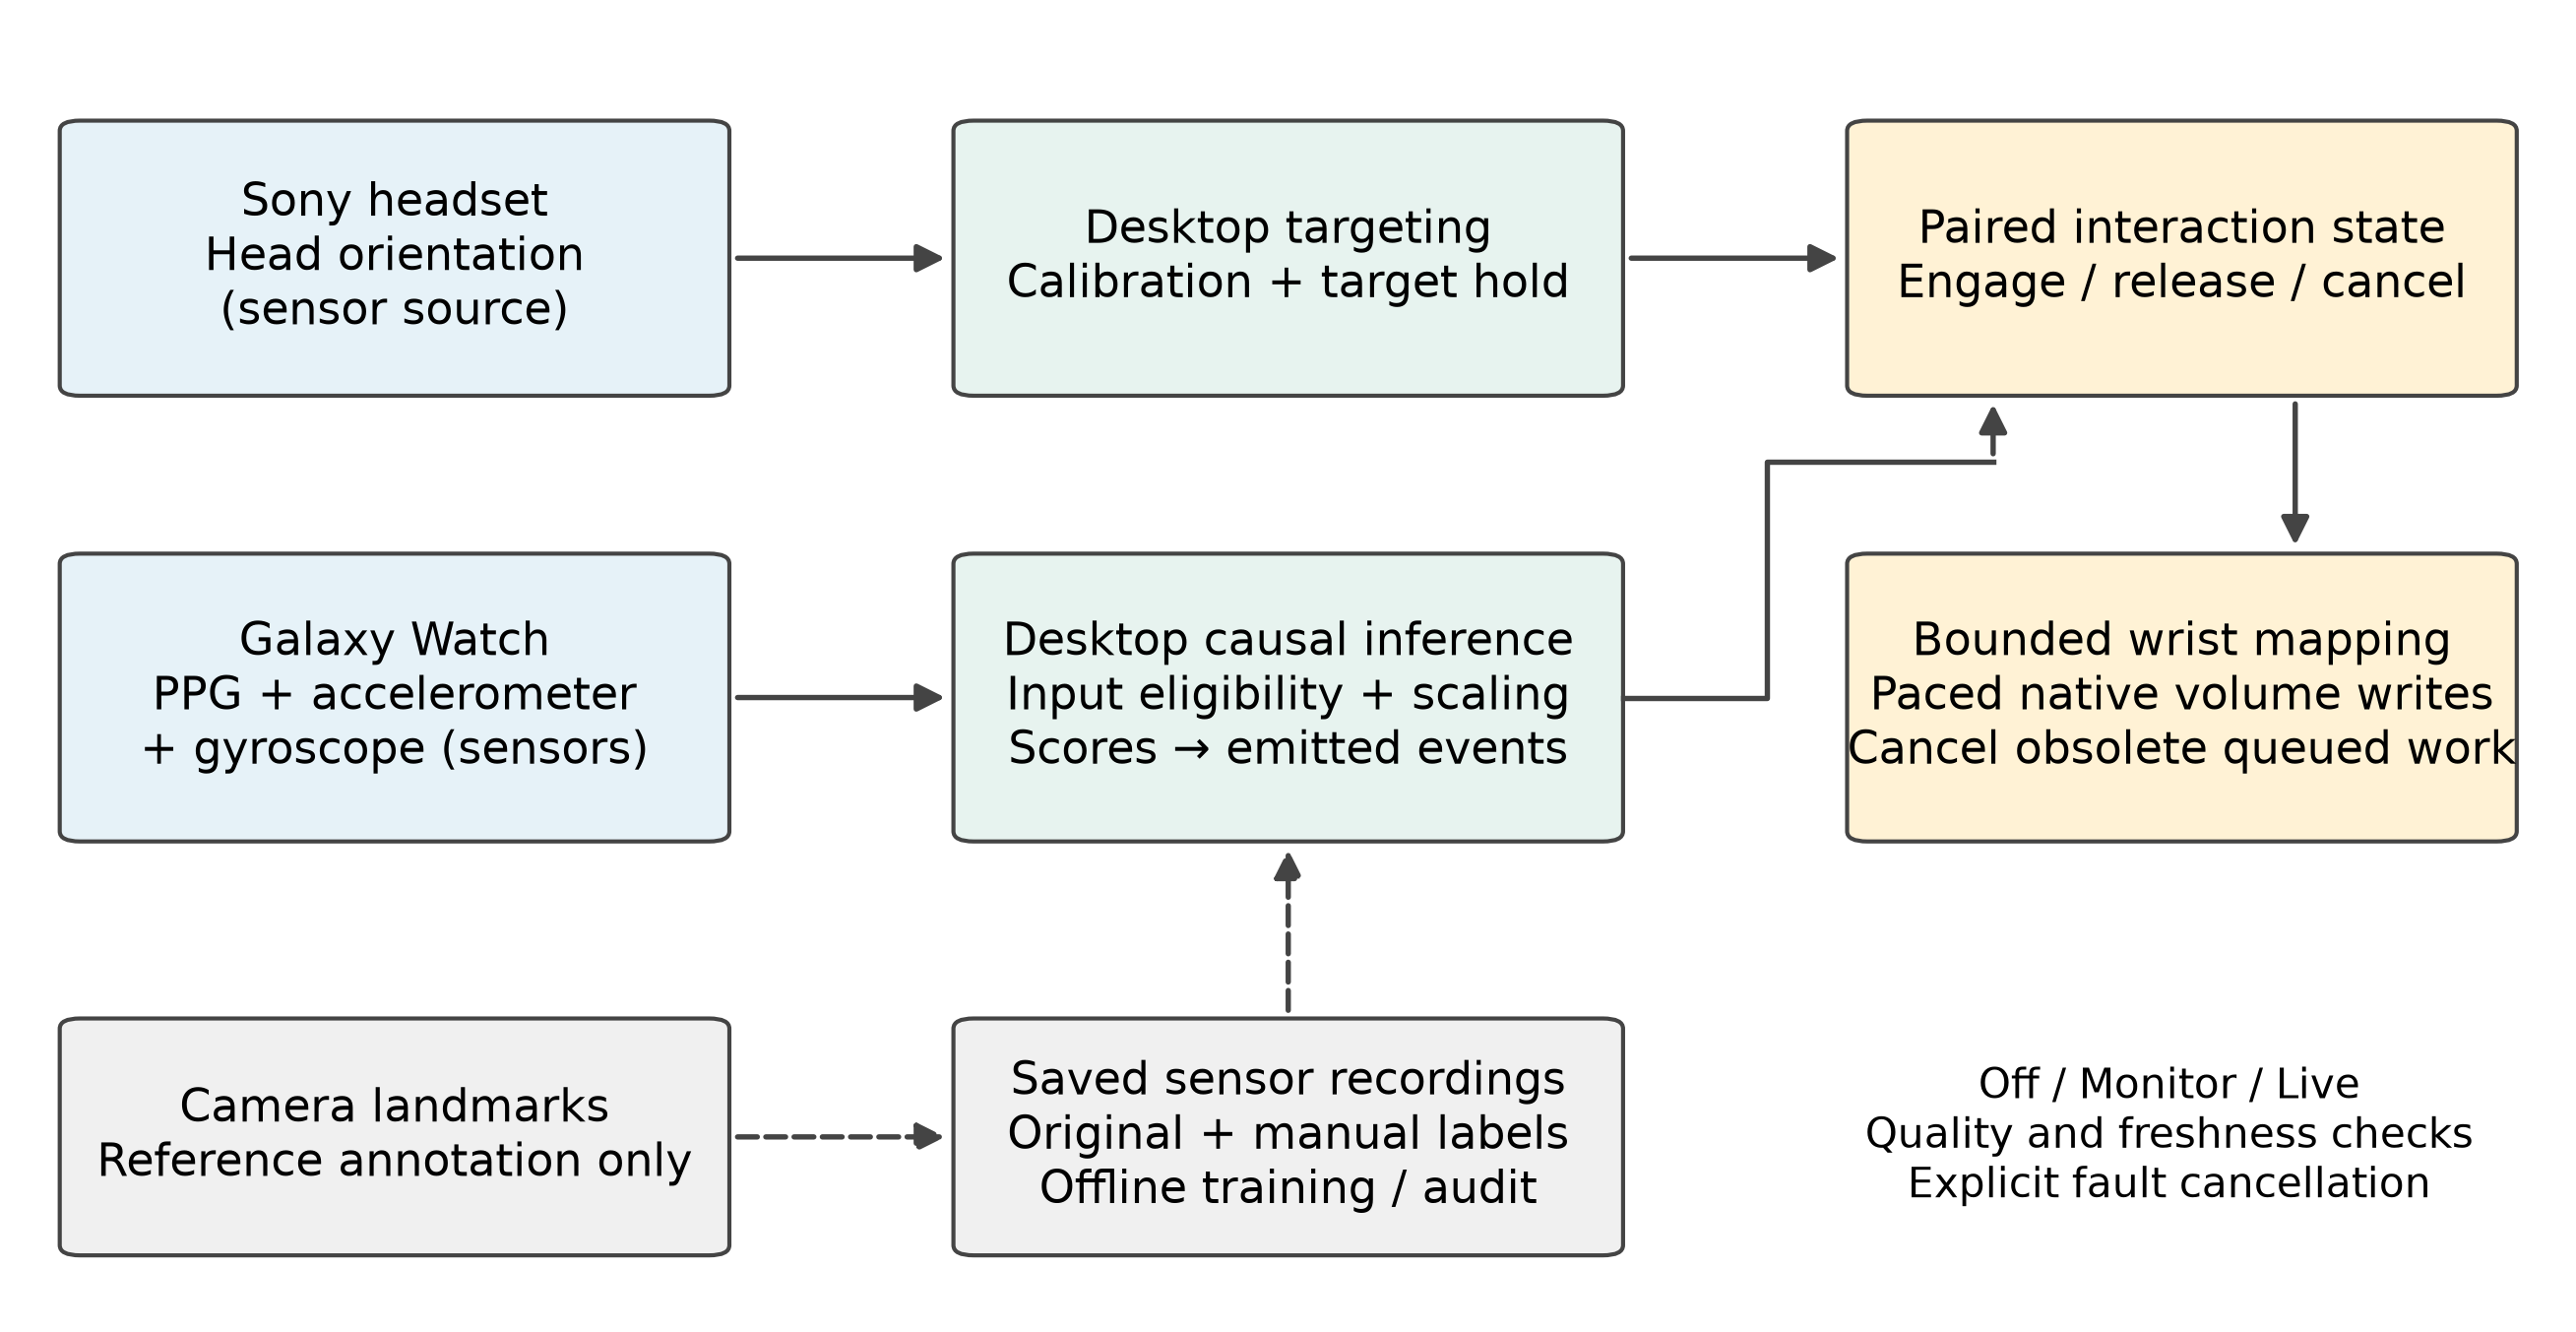
\includegraphics[width=1\linewidth,height=\textheight,keepaspectratio,alt={System architecture: headphone orientation supplies target selection, watch PPG and IMU supply desktop causal inference, and a paired interaction policy controls bounded volume writes; camera reference annotation is an offline path.}]{figures/system-overview.png}
\caption[System overview]{System overview. Head orientation selects the target, watch PPG and IMU feed a causal detector on the laptop, and a paired grab/release policy drives bounded volume changes. The camera is used only to create reference labels.}\label{fig-system}
\end{widefigure}

\subsect{Head targeting and paired interaction}\label{head-targeting-and-paired-interaction}

Head orientation is mapped to a calibrated point on the screen. This is head-directed selection; we do not track the eyes. While the head rests on the volume target, a fresh pinch-in event starts a grab. Wrist roll relative to the grab position then sets an absolute volume level, and a separate pinch-out event ends the grab. Silence from the detector is never taken to mean the fingers have opened, and further pinch-in events during a grab are ignored.

\iffull
The reason for this split is that a pinch is a momentary event, while adjusting the volume takes time. Letting one classifier score drive the output directly would tie the two together. Instead, recognition, interaction state and cancellation are handled separately. A grab also ends when the head leaves the target, when the user presses Escape, when the data become stale or are rejected, when the mode changes or when the model is replaced. If a start and a release arrive together, the release wins.
\else
Because a pinch is momentary while adjusting the volume takes time, recognition, interaction state and cancellation are handled separately. A grab also ends when the head leaves the target, on Escape, on stale or rejected data, on a mode change or on model replacement, and a simultaneous release beats a start.
\fi

\subsect{Bounded actuation and failure handling}\label{bounded-actuation-and-failure-handling}

\iffull
The application has three modes: Off, Monitor and Live. Monitor shows what the system would do without touching the system volume, and a saved Live setting is lowered to Monitor at startup, so the system never acts on its own after a restart. All output goes through the interaction policy; the web view cannot inject gesture events directly. Each model is checked against its declared hash and input format before loading. A matching hash shows the file is intact, not that the model works well.
\else
Off, Monitor and Live modes control actuation: Monitor shows what the system would do without changing the volume, and a saved Live setting starts as Monitor. All output passes through the interaction policy, and each model is checked against its declared hash and input format before loading. The wrist mapper bounds the rate and range of change, and queued volume writes are tagged with their grab so stale writes are discarded; a write already sent to the operating system still completes.
\fi

\iffull
The wrist mapper records a reference angle when the grab starts, limits how fast the level can change and clamps it to the valid range. Every queued volume write is tagged with the grab it belongs to, so writes left over from an earlier grab are discarded. A write that has already reached the operating system will still complete, so cancellation stops further changes rather than undoing the last one. Long-run transport reliability, battery use and cancellation timing on real hardware still need to be measured.

\fi
% Report-only chapter: implementation detail the paper has no room for.
% Sources: docs/architecture/*.md, docs/protocols/watch-*.md, apps/watch/README.md,
% tools/label-trainer/README.md, docs/performance.md, crates/interaction-engine.
\chapter{Implementation}\label{ch:implementation}

This chapter describes how the system is built: the components and how they communicate, the watch application, the two watch transports, head tracking, the desktop application, the recording and labelling tools, model training and the run-time inference and interaction engine.

\section{Overall Architecture}

The system has four deployable parts (Table~\ref{tab:components}). The watch and the headphones only supply sensor data; training, inference, interaction decisions and every action take place on the desktop.

\begin{table}[htbp]
\centering
\caption{Deployable components.}\label{tab:components}
\begin{tabularx}{\linewidth}{@{}l>{\raggedright\arraybackslash}X>{\raggedright\arraybackslash}X@{}}
\toprule
\textbf{Component} & \textbf{Runs on} & \textbf{Ships as} \\
\midrule
Desktop application & macOS, Windows, Linux (development) & A Tauri bundle per operating system \\
Galaxy Watch application & Wear OS 3 or later & An APK installed over \texttt{adb} \\
Sony head-tracker provider & The same computer as the desktop application & Linked into the desktop binary on macOS and Windows; a separate process on Linux \\
Per-label trainer & A developer checkout & Not shipped; the desktop runs it through \texttt{uv} \\
\bottomrule
\end{tabularx}
\end{table}

The desktop backend is a Rust workspace split into crates with one job each: wire types (\texttt{protocol}), head tracking (\texttt{head-tracking}, \texttt{native-head-tracking}), watch transport (\texttt{watch-bridge}), feature extraction and model execution (\texttt{pinch-inference}, \texttt{label-inference}), interaction logic (\texttt{interaction-engine}) and native volume control (\texttt{volume-control}). The Tauri backend wires them together and talks to the React front end through Tauri events and commands. A second, transparent, always-on-top window shows the volume knob during a grab.

Several background tasks run in the backend. The watch event loop routes every incoming message. A watchdog checks every 200\,ms and force-releases any grab whose model data have been stale for 750\,ms. A time-sync task estimates the watch--desktop clock offset every 5\,s for display; it is never applied to samples. A dedicated thread applies volume changes, at most one write every 100\,ms, so that slow operating-system calls never block the event loop.

\section{Watch Application}

The watch application is a self-contained Kotlin project for Wear OS. It streams the rotation vector (as a quaternion), accelerometer and gyroscope readings, and on a Galaxy Watch4 or later, raw green, red and infrared PPG from the Samsung Health Sensor SDK. It also answers time-sync requests from the desktop immediately and sends a heartbeat once a second.

Battery life shaped much of the design. Sensors, PPG and the CPU wake lock run only while a desktop is connected and receiving. While the app is waiting for a desktop, it keeps a foreground service so that Samsung's background process freezer does not suspend it, but it releases every sensor and the wake lock. The standard off-body sensor pauses collection when the watch is taken off. PPG is sent whenever the SDK delivers samples, instead of on a fixed polling timer, and orientation messages are encoded with a plain string builder, which a JVM benchmark measured as eight times faster than the earlier JSON-object encoder (0.4 against 3.2\,µs per message).

\section{Watch--Desktop Transport}

The watch reaches the desktop over one of two transports, chosen on the watch and mirrored in the desktop settings. Exactly one is active at a time, and a failing transport reports its error instead of silently falling back to the other.

\paragraph{Bluetooth Low Energy (default).} The watch is the GATT peripheral and the desktop the central, because the Rust Bluetooth library (btleplug) supports only the central role and that role behaves the same on macOS, Windows and Linux. The service exposes a telemetry characteristic (watch to desktop, notify) and a command characteristic (desktop to watch, write with response). Both require an encrypted, bonded link, and the watch sends nothing until the user taps \emph{Trust this computer}. Over Bluetooth the desktop assigns the device identity from the peripheral it discovered, so a watch cannot choose or spoof its identity.

\paragraph{Wi-Fi.} The desktop runs a WebSocket server on port 8766, and the watch finds it through mDNS. This path is intended for a trusted local network only: it uses plain \texttt{ws://} with no encryption or authentication.

\paragraph{Message layer.} Both transports carry the same UTF-8 JSON envelopes with a type, protocol version, device identifier, sequence number, watch timestamp in nanoseconds and payload, and the desktop decodes both through one function. Timestamps use the watch's boot-relative clock. Freshness and dwell decisions are always made on the desktop's own monotonic clock.

\paragraph{Performance under load.} Profiling on real hardware showed the original Bluetooth path sending about 61 notifications a second, one per motion reading, with the send queue growing to 512 fragments (several seconds of delay) before it was dropped all at once. Batching motion readings into 100\,ms packets halved the notification rate to about 30 a second. The send queue now holds about 0.5\,s and drops the oldest unsent messages first. In a 15-minute streaming test, 20 messages (about 2\,s of data) were lost, mostly right after connecting. A fragment-size bug that made Android reject every PPG packet at a 517-byte MTU was also fixed.

Figure~\ref{fig:sensor-timing} shows the timing of the data that actually reached the desktop, measured from the watch timestamps in the 28 distinct recordings used to train and evaluate the hand-labelled model. Inertial samples arrive at a steady 100\,Hz: the median interval is 10.0\,ms and 99\% of intervals are within 10.1\,ms. PPG samples average 25\,Hz (median 40.0\,ms), but their individual intervals spread widely, up to 97\,ms. PPG reaches the app in batches from the Samsung sensor service, flushed up to ten times a second, and the timestamps within those batches are uneven. The model's fixed 20\,ms grid with zero-order hold absorbs this jitter, and no interval in either stream came near the 250\,ms gap that marks an input as unavailable.

\begin{figure}[htbp]
\centering
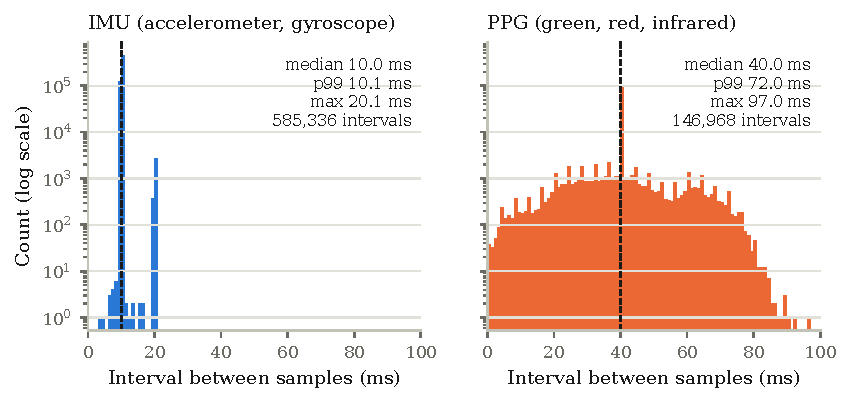
\includegraphics[width=\linewidth]{figures/sensor-timing.pdf}
\caption[Sample timing of the watch streams]{Intervals between consecutive samples, from watch timestamps in the 28 distinct recordings of the hand-labelled model. Dashed lines mark the nominal 10\,ms (IMU) and 40\,ms (PPG) periods. Log scale.}\label{fig:sensor-timing}
\end{figure}

\section{Head Tracking}

Head orientation comes from the motion sensors in Sony headphones. On macOS and Windows a native provider reads them in-process (through IOKit and IOBluetooth on macOS, HID and SetupAPI on Windows); on Linux, or when configured, an external command-line bridge sends JSON over loopback UDP to port 4243. Both feed the same provider interface.

Calibration stores a quaternion for the screen centre and for each target. At run time the engine measures the quaternion angular distance to each target and activates the nearest one after the head has stayed within 12° of it for 400\,ms. If the headphones reset their orientation reference, the calibration is invalidated and must be redone.

\section{Desktop Application}

The desktop application provides the live view of sensor streams, settings, calibration, the Recorder, Model Lab for training and managing models, and the inference mode switch (Off, Monitor, Live). A readiness indicator shows whether a pinch would be caught at that moment; after strong motion the CNN needs the wrist to be calm for about a second before it can catch a pinch again, and the indicator makes that visible.

All user state lives in the operating system's application directories: settings, recordings, datasets, the label catalogue, model bundles and the model registry. Writes that matter are atomic, and a corrupt registry file is reported as an error and left untouched instead of being replaced with an empty one.

\section{Recording and Labelling Tool}

The Recorder saves each session as an immutable bundle containing the raw sensor CSV, a metadata file and an annotations file. Bundles are staged and then renamed into place, so a crash never leaves a half-written recording, and they are never rewritten.

The Recorder can also save hand landmarks from the laptop camera. MediaPipe's Hand Landmarker runs inside the application's own web view, with its model and WebAssembly runtime served from the application's files; it finds 21 landmarks per hand in each frame. Only landmarks are saved, never images, and the application's content security policy blocks MediaPipe's attempt to send usage logs. To line the camera up with the watch, the Recorder logs pairs of watch timestamps and browser arrival times about every 200\,ms; on export, each camera frame is placed on the watch clock using the smallest arrival offset in the recording.

Exported datasets contain \texttt{ppg.csv} and \texttt{imu.csv}, plus the landmark and clock-sync files when a camera was used. Each sample keeps its original \texttt{label} column, and manual corrections go in a separate \texttt{manual\_label} column, following the rules described in Section~\ref{effective-label-semantics}.

\section{Model Training Pipeline}

Training runs offline in the Python \texttt{label-trainer}. The desktop decides everything that must be fixed in advance (which recordings train and which evaluate, never the same one, and what each label means: target, negative or left out) and passes it to the trainer in a specification file.

The trainer supports two model families:
\begin{itemize}
\item \textbf{ExtraTrees} (300 trees) on engineered features. The PPG-only version uses 1,701 features: each PPG channel is z-scored against the previous 1, 2 and 4\,s, its slope, curvature and jerk are estimated with a local cubic fit, and 21 statistics are taken over the last 8, 16 and 32 ticks of a 25\,Hz grid. The PPG+IMU version adds 1,032 motion features, for 2,733 in total. It fires about 0.9\,s after a pinch starts.
\item \textbf{CNN} on 450 inputs (nine channels by 50 ticks of a 50\,Hz grid), described in Section~\ref{models-and-learning-configuration}. It fires about 0.5\,s after a pinch starts.
\end{itemize}

The decision threshold is fitted on the training recordings, each scored by a model trained without it. The trainer then replays the model over every held-out recording through the same detection rule the runtime uses, and reports starts caught, delay and false activations per hour. The model is written as plain data (tree node arrays or JSON weights), never as executable code. A model that does not pass the checks for going live is still written, but as evaluation-only: the desktop can activate it in Monitor mode, where it only reports.

The same feature code exists twice, in Python for training and in Rust for live use. Shared test fixtures keep the two implementations numerically equal, so a model sees the same inputs in use as in training.

\section{Desktop Inference and Interaction Engine}

\paragraph{Model loading.} A model bundle is a manifest plus one model file. Before a model is loaded the runtime checks the manifest's schema, sources, feature names and order, input shape, window and file format; it checks that the file's SHA-256 matches the manifest, that the network's layers chain and its weights are finite, and that the model returns a probability on four constant test inputs. Only a registry version that is Active, and whose hash is the approved one, is loaded. The tree ensembles and the CNN are both evaluated in Rust, in-process, with no Python at run time.

\paragraph{Decision chain.} Each incoming PPG batch passes through an ordering check, a quality gate, a window check, fusion with recent orientation, feature extraction and the model, and the result goes to the gesture policy. Any stage that rejects a window forces a release of an open grab. Fusion rejects orientation older than 500\,ms, data from the wrong device and non-finite or out-of-order values.

\paragraph{Gesture policy.} The policy is a state machine that turns model events into the \texttt{VolumeGrab} and \texttt{VolumeRelease} intents, but only in Live mode and only for the intents explicitly bound to the active model. It ends a grab on a pinch-out, when the head leaves the target, on Escape, on stale or rejected data, on a mode change or when the model is replaced; a release that arrives together with a start wins.

\paragraph{Wrist mapper and volume writer.} At the start of a grab the mapper records the current wrist roll. Changes smaller than a 3° dead zone are ignored; beyond it, every 3° of roll moves the volume by one point, limited to 30 points a second and clamped to the valid range. A reading that implies rotation faster than 360°/s is treated as noise and ignored. Volume writes go to native back ends: Core Audio on Windows, the system volume on macOS, and \texttt{wpctl} or \texttt{pactl} on Linux. Each queued write is tagged with the grab it belongs to, so writes left over from a finished grab are discarded. Figure~\ref{fig:wrist-mapping} shows the mapping and the effect of the rate limit on a fast turn.

\begin{figure}[htbp]
\centering
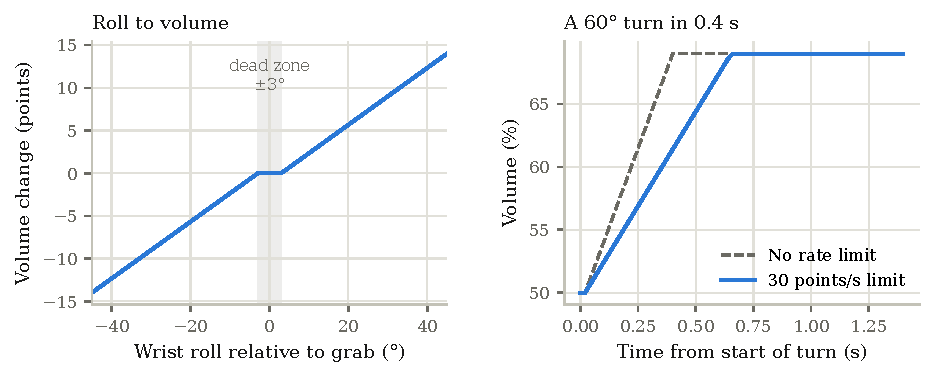
\includegraphics[width=\linewidth]{figures/wrist-mapping.pdf}
\caption[Wrist-roll to volume mapping]{Wrist-roll mapping with the default settings. Left: volume change against roll relative to the grab angle, with the $\pm3^\circ$ dead zone. Right: a simulated 60° turn made in 0.4\,s from volume 50, sampled at 50\,Hz; the 30 points/s limit stretches the change to about 0.65\,s. Computed from the interaction engine's default configuration.}\label{fig:wrist-mapping}
\end{figure}

% Shared section: used by paper-ieee.tex, paper-lncs.tex and report.tex.
% Use \sect / \subsect for headings (see README), never \section directly.

\sect{Reference Annotations and Source Audit}\label{reference-annotations-and-source-audit}

\iffull
\subsect{Evidence cohorts}\label{evidence-cohorts}
\fi

\iffull
The project's data fall into three groups. Older experiments used cue labels or automatic labels from camera landmarks. Later recordings carry manually corrected labels. A future confirmatory test would use new recordings collected only after the model and protocol are frozen. Results from one group cannot stand in for another; adding corrected labels to a folder does not change the labels a historical result was computed with.
\else
Recordings fall into three groups: older ones with cue or automatic camera labels, later ones with manually corrected labels, and future recordings for a frozen confirmatory test. Each sample keeps its original \nolinkurl{label}; a non-empty \nolinkurl{manual_label} replaces it, a blank one keeps it, and \nolinkurl{-} removes it. A script that reads only the original column silently ignores the corrections, so every result must name its loader and label version.
\fi

\iffull
All recordings come from one participant, the author, wearing the watch on the left wrist. The audit covers the recordings and models stored in the project, not a wider population. Raw sensor values are never modified; label corrections are stored alongside the original labels.
\fi

\iffull
\subsect{Effective-label semantics}\label{effective-label-semantics}
\fi

\iffull
Each sample has an original \nolinkurl{label} and an optional \nolinkurl{manual_label}. A non-empty manual label replaces the original; a blank one keeps it; the marker \nolinkurl{-} removes it. The label \nolinkurl{left_out} marks a stretch that may be excluded, but whether it is excluded depends on the experiment's configuration. It should not quietly turn into a negative example, or vanish from the no-gesture time, without a stated rule.
\fi

\iffull
These rules guard against two mistakes. A blank manual field does not mean someone checked the sample and found no gesture. And an older script that reads only the \nolinkurl{label} column will ignore the corrections even when it runs on a newer file. Every result therefore has to name the loader and evaluator it used as well as the label version. Unit tests confirm that the override and fallback rules work; they cannot tell us whether the human-drawn boundaries are correct.
\fi

\begin{widefigure}
\centering
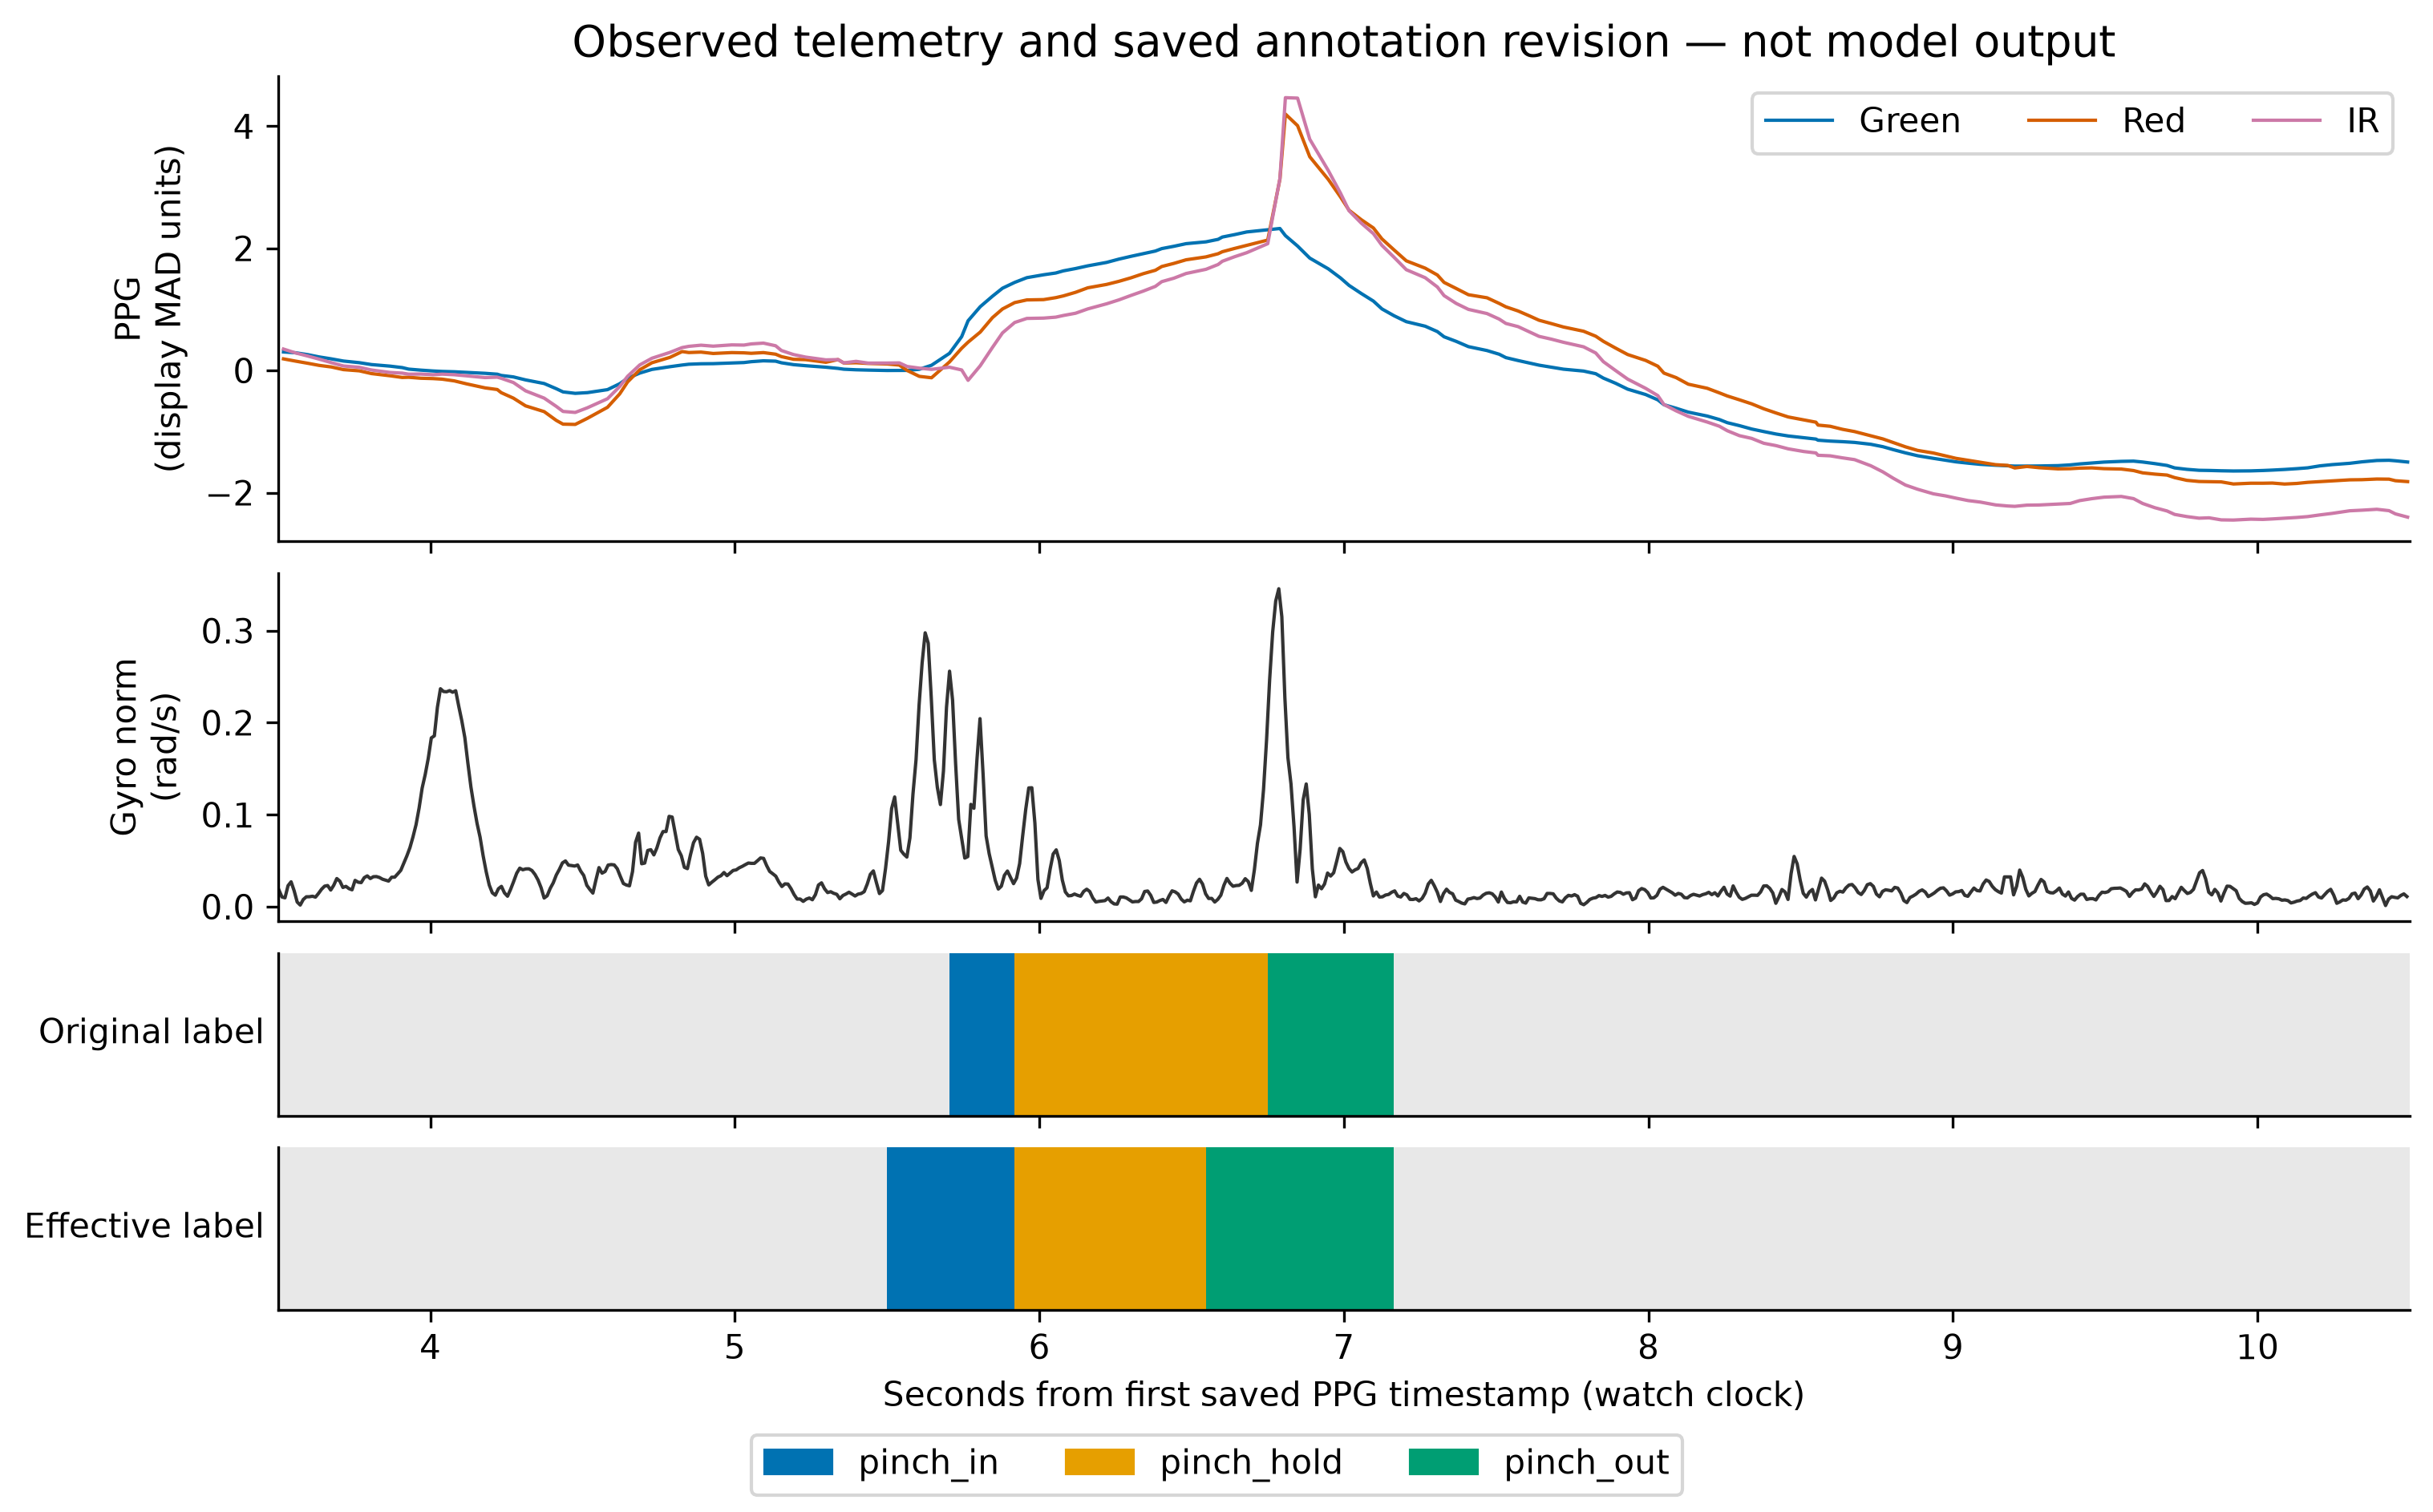
\includegraphics[width=1\linewidth,height=\textheight,keepaspectratio,alt={Saved optical and gyroscope data with original and effective row-label bands from a manually revised recording.}]{figures/annotation-telemetry.png}
\caption[Recorded PPG and gyroscope data with original and corrected labels]{Recorded PPG and gyroscope data from \nolinkurl{gesture-dataset-pinch_hold-2026-11-03T01-05-59.434Z}, with original and corrected label bands. Time is relative to the first PPG sample on the watch clock. For display only, each PPG channel is centred on its median and scaled by its MAD; gyroscope magnitude is in rad/s. No model output is shown.}\label{fig-annotation}
\end{widefigure}

\iffull
\subsect{Audit method}\label{audit-method}
\fi

\iffull
The audit reads every PPG and IMU file in the hand-labelled folder without changing anything. For each stream it hashes the ordered sensor columns, leaving out the label columns so that relabelled copies of the same data still match. The pair of PPG and IMU hashes identifies a source stream. We then match export names and recording IDs against the training and evaluation lists in each model manifest, and check each model file against its declared SHA-256.
\else
To find duplicates, we hashed each recording's ordered sensor columns, leaving out the labels, and used the pair of PPG and IMU hashes as the stream's identity. This catches exact copies but not partial overlaps.
\fi

\iffull
This finds exact duplicates only. Two crops of the same session, partial overlaps or a file saved in a different format would not match. Grouping by source is necessary for a clean split, but it cannot prove that days or sessions are independent, nor rule out repeated model selection on the evaluation data. The audit scripts, full inventory and figure sources are kept with the project artifacts (Section~\ref{limitations-and-reproducibility}).
\fi

\iffull
\subsect{Dataset identity findings}\label{dataset-identity-findings}
\fi

\iffull
The folder holds 37 exports totalling 127.918 minutes of PPG. Nine pairs of exports contain identical PPG and IMU streams under different names, which leaves 28 distinct streams and 98.080 minutes. This is total recording time after removing duplicates; it is not the same as independently collected sessions or no-gesture exposure. Six of the duplicate pairs carry pinch-hold and pinch-in names, and three carry supported and unlabelled names.
\else
The hand-labelled folder holds 37 exports (127.918 minutes of PPG), but nine pairs are identical streams under different names, leaving 28 distinct streams (98.080 minutes). Fourteen exports carry manual labels, which change the label of 4,931 PPG samples (Table~\ref{tab-audit}).
\fi

\iffull
Fourteen exports contain manual labels on PPG samples. Across all 37 exports, 4,931 PPG samples have a corrected label that differs from the original. That is a count of samples, not of editing actions or gesture events. Being in the folder does not prove a recording was reviewed, and an absent override does not prove it was not; reviews were not logged.
\fi

\begin{table}[t]
\centering\small
\caption[Hand-labelled folder audit]{Hand-labelled folder audit. Counts refer to exported files or exact stream pairs, not independent sessions.}\label{tab-audit}
\begin{tabularx}{\linewidth}{@{}>{\raggedright\arraybackslash}Xr>{\raggedright\arraybackslash}X@{}}
\toprule
\textbf{Quantity} & \textbf{Count} & \textbf{Note} \\
\midrule
Exported directories & 37 & Includes duplicates \\
Distinct stream pairs & 28 & Exact matches only \\
Duplicate pairs & 9 & Must share a split \\
Exports with PPG overrides & 14 & Review coverage unknown \\
PPG samples relabelled & 4,931 & Samples, not events \\
\bottomrule
\end{tabularx}
\end{table}

\iffull
For the hand-labelled pinch-in model, all 20 training and 8 evaluation IDs resolve to recordings in the folder. The two sets do not overlap, and no stream appears in both. So the duplicates we found did not leak into this particular split. Other median-model manifests use UUIDs that we could not map to the folder's metadata, so their splits remain unchecked.

\else
For the hand-labelled pinch-in model, the 20 training and 8 evaluation recordings share no stream, so these duplicates did not leak into its split.
\fi
% Shared section: used by paper-ieee.tex, paper-lncs.tex and report.tex.
% Use \sect / \subsect for headings (see README), never \section directly.

\sect{Causal Detection and Event Accounting}\label{causal-detection-and-event-accounting}

\iffull
\subsect{Median-scaled optical--inertial input}\label{median-scaled-opticalinertial-input}
\fi

The model takes nine channels: three axes each of acceleration and angular velocity, and three PPG wavelengths. At decision time \(T\), each channel is placed on a 20\,ms grid by zero-order hold, using only samples recorded at or before each tick. The grid has 549 ticks ending at \(T\), spanning 10.96\,s of an 11\,s history window. The last 50 ticks form the model input, flattened channel by channel into 450 values.

Let \(G_T\) be the grid, \(W_T\) its last 50 ticks, and \(c\) a channel. We define
\[
m_c(T)=\operatorname{median}_{j\in G_T}x_{c,j},
\]
\[
s_c(T)=1.4826\operatorname{median}_{j\in G_T}|x_{c,j}-m_c(T)|,
\]
\[
u_{c,t}=\sigma\left(\operatorname{clip}\left(\frac{x_{c,t}-m_c(T)}{s_c(T)+\epsilon_c(T)},-500,500\right)\right),\quad t\in W_T.
\]

\iffull
The floor \(\epsilon_c\) is 0.02\,m/s² for acceleration, 0.01\,rad/s for angular velocity and \(0.001(|m_c(T)|+1)\) for PPG. A single centre and spread is computed over the whole grid at each decision, so the transform uses only past data. If the history is too short or contains a large gap, the input is marked unavailable instead of being scored as a negative. The scaling used for display in Fig.~\ref{fig-annotation} is different and should not be confused with this transform.
\else
The floor \(\epsilon_c\) is 0.02\,m/s² for acceleration, 0.01\,rad/s for angular velocity and \(0.001(|m_c(T)|+1)\) for PPG. The transform uses only past data, and an input with too little history or a large gap is marked unavailable rather than scored as a negative.
\fi

\iffull
Earlier models used a rolling ten-second mean and standard deviation ending at each tick. Each model declares its preprocessing type, and that declaration, not the free-text description, decides which transform applies. Some median-model manifests still describe the rolling pipeline in their provenance text; this is an exporter bug that needs fixing, and we have not relabelled the old results.
\fi

\iffull
\subsect{Models and learning configuration}\label{models-and-learning-configuration}
\fi

\iffull
The CNN, written in PyTorch \cite{pytorch}, has three dilated convolutions \cite{yu2016dilated,bai2018tcn} with 32, 32 and 64 channels, kernel width five and dilations of one, two and four. Batch normalisation \cite{ioffe2015batchnorm} is followed by max and mean pooling, a 32-unit dense layer and a single binary output. The trainer can average three models trained with different seeds. Its default configuration trains for twelve epochs with Adam \cite{kingma2015adam} (learning rate 0.001, weight decay 0.0001) in batches of 256. Positive training examples are taken 0.4--0.6\,s after an annotated pinch start; negatives and class weights follow the trainer configuration.
\else
The CNN, written in PyTorch \cite{pytorch}, has three dilated convolutions \cite{yu2016dilated,bai2018tcn} (32, 32 and 64 channels, kernel width five, dilations one, two and four), batch normalisation \cite{ioffe2015batchnorm}, max and mean pooling, a 32-unit dense layer and a binary output. It is trained for twelve epochs with Adam \cite{kingma2015adam} (learning rate 0.001, weight decay 0.0001, batches of 256), with positive examples taken 0.4--0.6\,s after an annotated start. An ExtraTrees model on engineered features \cite{geurts2006extra,sklearn} also exists but has not yet been compared on the corrected labels.
\fi

\iffull
This is the documented default, not a full training log for every model. The hand-labelled model records twelve epochs, seed 17 and its convolution widths, but not its complete sampling or ensemble-selection history. The project also includes an ExtraTrees model on engineered features \cite{geurts2006extra,sklearn}; we have not yet compared it with the CNN on the corrected labels.
\fi

\iffull
\subsect{From scores to emitted events}\label{from-scores-to-emitted-events}
\fi

\iffull
The detector turns the score stream into events using an activation threshold and a lower release threshold. Once the score passes the activation threshold, an event is emitted at the first decision where the score falls, so the event time is when the peak was confirmed, not the peak itself. The detection ends when the score drops below the release threshold, and a cooldown then blocks an immediate retrigger. Latency is measured from the emitted time.
\else
Events come from hysteresis on the score. Once it passes the activation threshold, an event is emitted at the first decision where the score falls; the detection ends below the release threshold, and a cooldown blocks retriggering. For the hand-labelled model these are 0.99, 0.84 and 1,500\,ms, with a nominal decision delay of 500\,ms. Latency is measured from the emitted time.
\fi

\iffull
For the hand-labelled pinch-in model, the activation threshold is 0.99, the release threshold 0.84 and the cooldown 1,500\,ms. Its nominal decision delay of 500\,ms is a training and scoring setting, not a measured sensor-to-action latency. These values belong to this model and should not be carried over to the historical comparisons.
\fi

\iffull
\subsect{Continuous metrics and eligibility}\label{continuous-metrics-and-eligibility}
\fi

\iffull
We score each detector over whole recordings. An event that falls within the match window of an eligible annotated start is matched to it one-to-one. A second event during a gesture that was already caught is a repeat. An event during an uncaught gesture but outside its window is late. An event while no gesture is under way is a false activation. For the 500\,ms CNN delay, the match window runs from 300 to 900\,ms after the annotated start. Exclusions and event-merging rules are reported with each experiment.
\else
An event within 300--900\,ms after an eligible annotated start is matched to it one-to-one. A second event during a caught gesture is a repeat, an event during an uncaught gesture but outside its window is late, and any event while no gesture is under way is a false activation.
\fi

Event recall and false-activation rate are
\[
R_e=\frac{N_{\mathrm{caught}}}{N_{\mathrm{eligible\ starts}}},\qquad
\lambda_{\mathrm{FA}}=\frac{N_{\mathrm{false\ events}}}{T_{\mathrm{eligible\ no\ gesture}}/3600},
\]
with time in seconds. We also report misses, repeats, late events and latency. Window ROC AUC and window F1 are kept as diagnostics; they are not event-level measures.

\iffull
The exposure calculation needs care. The evaluator takes the span from the first to the last eligible decision and subtracts gesture and excluded intervals, but it does not subtract gaps inside that span where no decisions were made. Such gaps would inflate the no-gesture time. For the hand-labelled model we rebuilt the decision timeline: decisions arrive every 40\,ms in all eight evaluation recordings, with no gap longer than 250\,ms, so its exposure is not inflated. The evaluator should still report coverage directly.

\else
We checked that gaps in the decision stream do not inflate the no-gesture time: decisions arrive every 40\,ms in all eight evaluation recordings, with no gap longer than 250\,ms.
\fi
% Shared section: used by paper-ieee.tex, paper-lncs.tex and report.tex.
% Use \sect / \subsect for headings (see README), never \section directly.

\sect{Results}\label{results}

\iffull
\subsect{Later hand-labelled development artifact}\label{later-hand-labelled-development-artifact}
\fi

\iffull
The hand-labelled model is \nolinkurl{pinch_in-ae0a22bf}, SHA-256 \nolinkurl{ae0a22bf8f744d5fa2fce9208221f0947288c5ba5c5eb196180985a70d77ba0d}. Its bytes match the manifest, as do those of all seven model files in the project. This confirms the files are intact; it does not tell us which model is running on any given laptop.
\else
We evaluate the hand-labelled pinch-in model \nolinkurl{pinch_in-ae0a22bf}, whose file matches its declared SHA-256. Its threshold was chosen on the training recordings, not on the evaluation set, and its stored window ROC AUC is 0.982.
\fi

\iffull
The manifest records a window ROC AUC of 0.981993, balanced accuracy of 0.881720 and window F1 of 0.865854, together with an event recall of 0.824561 and no false activations. The threshold was chosen on the training recordings (\nolinkurl{thresholdChosenOnEvaluationRecordings} is false). That is a stronger separation than tuning on the evaluation set, but the evaluation recordings may still have influenced label edits, architecture choices or which candidate model was kept.
\fi

\iffull
\begin{table}[t]
\centering\small
\caption[Stored manifest fields of the pinch-in model]{Stored manifest fields for the pinch-in model. The event values were reproduced by replay. These are development results, not a prospective test.}
\begin{tabularx}{\linewidth}{@{}>{\raggedright\arraybackslash}Xr>{\raggedright\arraybackslash}X@{}}
\toprule
\textbf{Field} & \textbf{Value} & \textbf{Status} \\
\midrule
Training IDs & 20 & All resolved \\
Evaluation IDs & 8 & All resolved \\
Event recall & 82.46\% (47/57) & Reproduced \\
False activations & 0 in 0.48 h & Reproduced \\
Window ROC AUC & 0.981993 & Window-level \\
Window F1 & 0.865854 & Window-level \\
\bottomrule
\end{tabularx}
\end{table}
\fi

\iffull
The model was saved without its event log, so we recovered it by replay. The exact training specification was not saved either. We rebuilt the label roles from the project's documented defaults and tried all four combinations of the two uncertain settings (whether \nolinkurl{left_out} is excluded, and whether the still-hand rule applies); all four gave the same result. Running the stored model over the eight evaluation recordings with the trainer's own input building, detection rule and event accounting reproduced the stored metrics exactly (Table~\ref{tab-replay}).
\else
The model was saved without its event log, so we recovered it by replaying the stored model over its eight evaluation recordings with the trainer's own code. This reproduced the stored metrics exactly (Table~\ref{tab-replay}).
\fi

\begin{table}[t]
\centering\small
\caption[Replayed event outcomes of the pinch-in model]{Replayed event outcomes of the hand-labelled pinch-in model on its eight evaluation recordings.}\label{tab-replay}
\begin{tabularx}{\linewidth}{@{}>{\raggedright\arraybackslash}Xr>{\raggedright\arraybackslash}X@{}}
\toprule
\textbf{Outcome} & \textbf{Value} & \textbf{Basis} \\
\midrule
Caught / eligible starts & 47 / 57 (82.5\%) & Matches manifest \\
By day (3, 4, 6 Nov) & 17/18, 17/21, 13/18 & Replay \\
Missed & 10 (4 late, 6 undetected) & Replay \\
Repeats; false activations & 0; 0 & Matches manifest \\
Eligible no-gesture time & 1,735.4 s (0.48 h) & Replay, no gaps \\
95\% upper false-activation rate & 6.2 per hour & Poisson, zero events \\
Latency, median (IQR; p95) & 442 ms (384--510; 649) & From emission \\
\bottomrule
\end{tabularx}
\end{table}

\iffull
Figure~\ref{fig:score-timeline} shows how this looks over time for one evaluation recording, the pinch-hold session of 4 November. Of its 21 annotated starts, 17 were caught. The other four show three different ways a pinch can be missed. One produced no response at all. One raised the score to 0.906, short of the 0.99 activation threshold. The remaining two produced an event about 280\,ms after the start, just before the 300\,ms match window opens; the evaluation counts these as late, although they came slightly early. Between pinches the score stays close to zero, and the recording has no false activations. Figure~\ref{fig:latency} shows the latencies of all 47 caught starts across the eight recordings: most fall between 350 and 550\,ms, with a tail up to 755\,ms.

\begin{figure}[htbp]
\centering
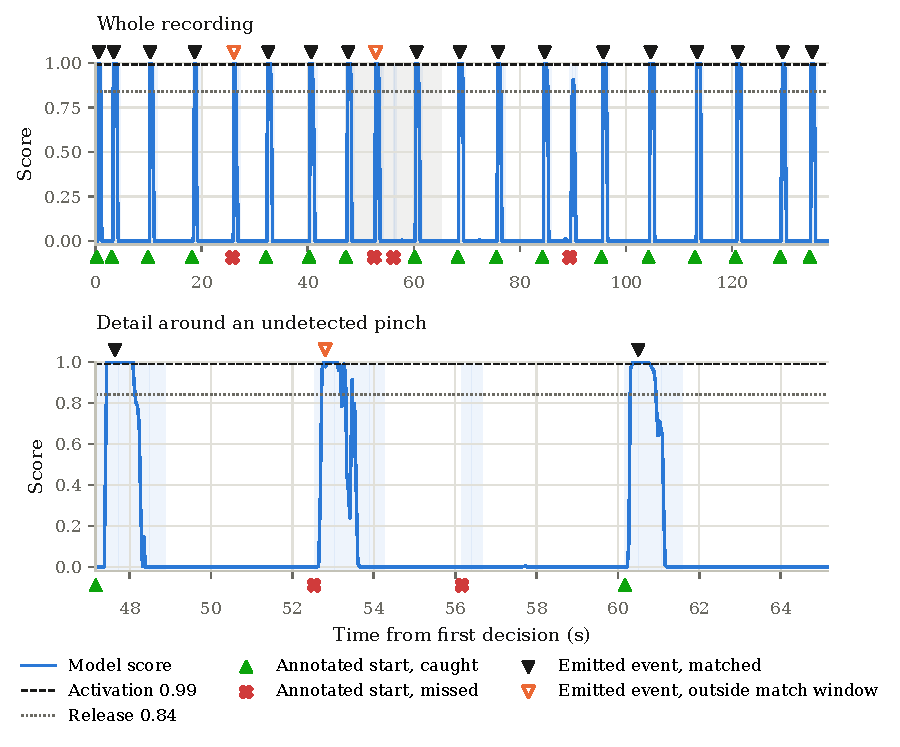
\includegraphics[width=\linewidth]{figures/score-timeline.pdf}
\caption[Model score over an evaluation recording]{Score of the hand-labelled pinch-in model over the evaluation recording \nolinkurl{gesture-dataset-pinch_hold-2026-11-04T04-50-33.518Z}, replayed with the trainer's own detection rule. Shaded bands are annotated pinch gestures; markers below the axis are annotated starts, markers above are emitted events. The grey region in the top panel is shown in detail below.}\label{fig:score-timeline}
\end{figure}

\begin{figure}[htbp]
\centering
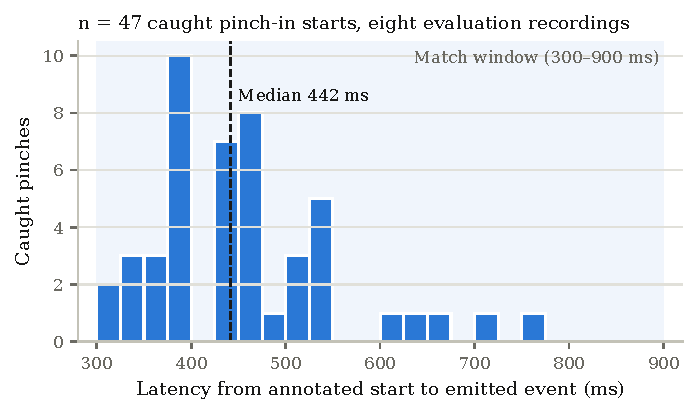
\includegraphics[width=0.85\linewidth]{figures/latency-histogram.pdf}
\caption[Latency of caught pinches]{Latency from the annotated start to the emitted event for the 47 caught pinch-in starts in the eight evaluation recordings (25\,ms bins). The shaded region is the 300--900\,ms match window.}\label{fig:latency}
\end{figure}
\fi

\iffull
Latency is measured from the annotated start to the moment the event is emitted. The margin behind the zero false-activation count is thin. In the everyday-activity recording the highest score reached 0.970, just under the 0.99 threshold; lowering the threshold to 0.98 would have added one false activation, and 0.95 would have added two. We report this as a sensitivity check, not as a reason to pick a different threshold.
\else
The margin behind the zero false-activation count is thin. In the everyday-activity recording the highest score reached 0.970 against the 0.99 threshold, and thresholds of 0.98 and 0.95 would have added one and two false activations.
\fi

\iffull
There is no hand-labelled pinch-out model. A median pinch-out model exists, but its training data cannot be traced, so it is not a matched counterpart. The result above therefore covers pinch-in only, not the full grab-and-release interaction.
\else
There is no matched hand-labelled pinch-out model, so these results cover pinch-in only.
\fi

\iffull
\subsect{Historical camera-label transfer}\label{historical-camera-label-transfer}
\fi

\iffull
The best historical configuration, trained on camera labels with noise recordings and without a still-hand gate and evaluated leave-one-day-out, caught 161 of 372 pinch-in starts (43.3\%). It produced seven false activations per hour on noise recordings and 49 per hour during no-gesture time inside pinch recordings. These rates use different denominators and should not be averaged.
\else
An earlier configuration trained on camera labels caught 161 of 372 pinch-in starts (43.3\%) under leave-one-day-out evaluation, with seven false activations per hour on noise recordings and 49 per hour within pinch recordings. Recall ranged from 21 of 171 on 14 October to 67 of 92 on 3 November (Fig.~\ref{fig-historical}), a spread that a pooled number hides.
\fi

\iffull
Performance varied widely by day: 21 of 171 on 14 October, 37 of 52 on 17 October, 67 of 92 on 3 November and 36 of 57 on 4 November (Fig.~\ref{fig-historical}). The later days support the earlier statement that the model catches about two thirds of unseen pinches; the pooled result does not. An earlier result of 204 of 372 came from a model trained on many October sessions and is not a clean October holdout.
\fi

\begin{widefigure}
\centering
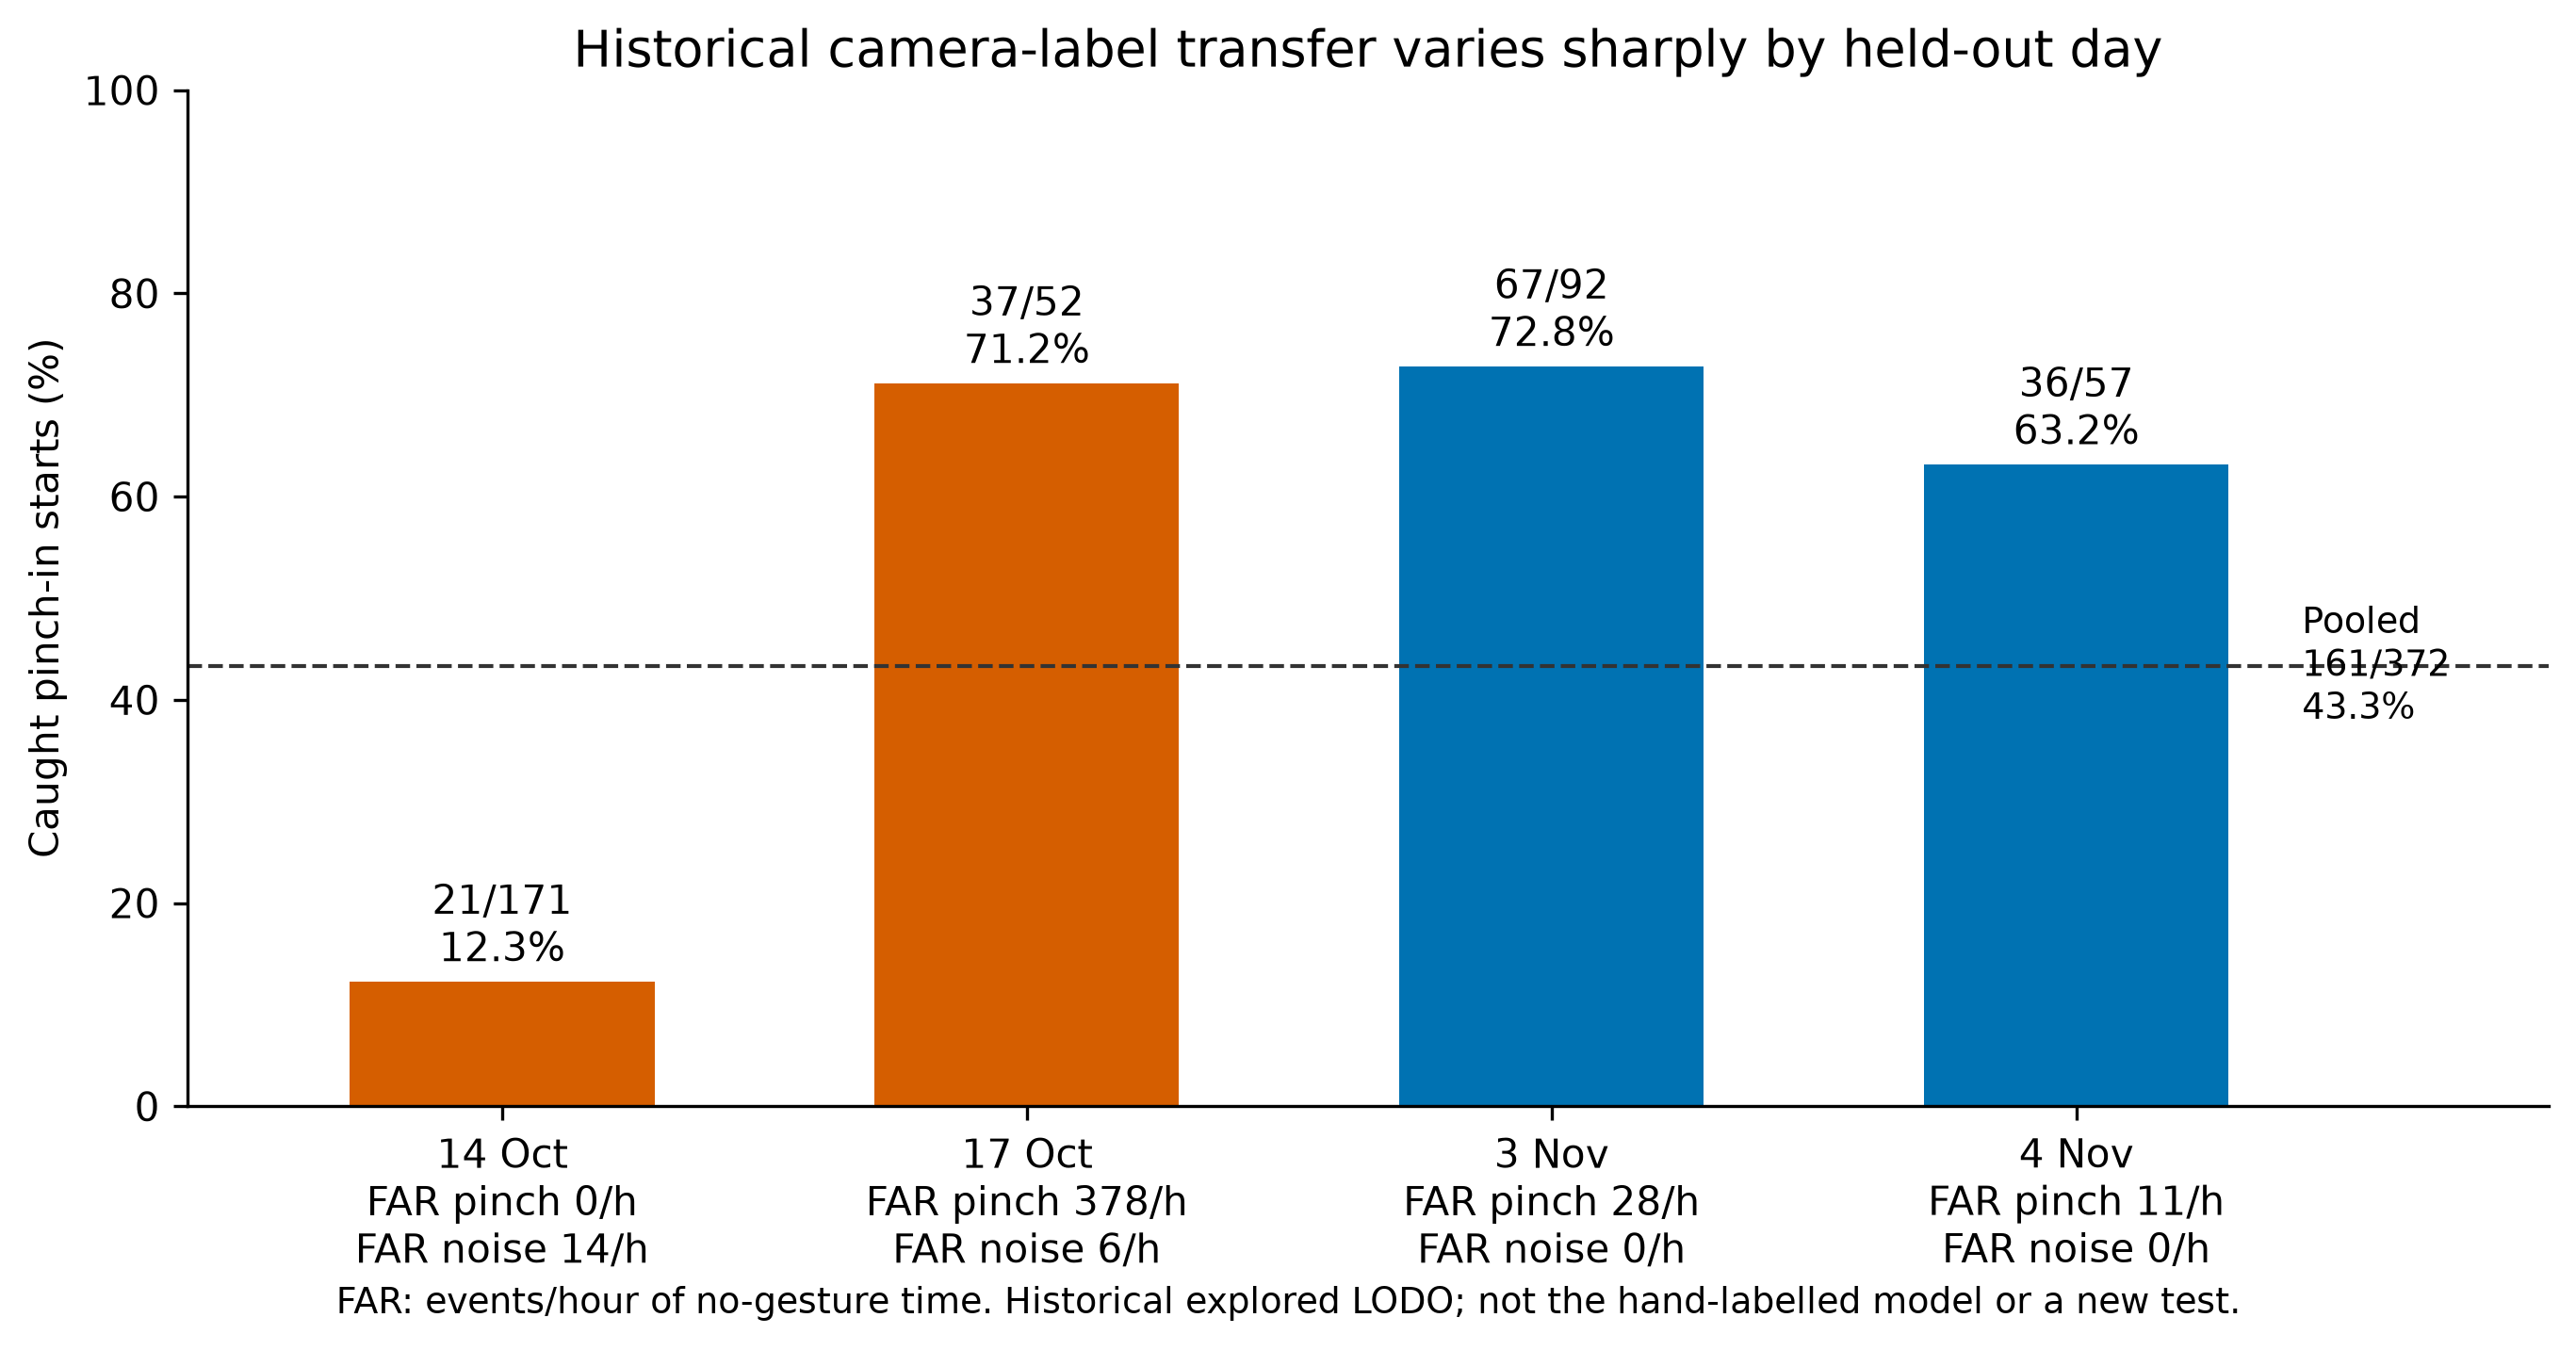
\includegraphics[width=1\linewidth,height=\textheight,keepaspectratio,alt={Historical day-level continuous recall and condition-specific false activations for the selected camera-labelled configuration.}]{figures/historical-day-transfer.png}
\caption[Historical camera-label results by day]{Historical camera-label results, leave-one-day-out. Bars show caught/eligible starts per day; the dashed line is the pooled 161/372. False-activation rates use each condition's own no-gesture time. All days come from one participant.}\label{fig-historical}
\end{widefigure}

\iffull
So, for RQ2: the stored files are intact, the hand-labelled pinch-in split is free of exact duplicates, and the stored development result can be reproduced. We cannot conclude that the manual relabelling improved recall over the older model, because the labels, recordings, preprocessing and thresholds all changed at once.
\else
For RQ2, the stored result is reproducible and its split is free of exact duplicates, but we cannot credit any gain to relabelling, because labels, recordings, preprocessing and thresholds all changed together.
\fi

\iffull
\subsect{Historical diagnostics, not current-model validation}\label{historical-diagnostics-not-current-model-validation}
\fi

\iffull
Earlier fusion experiments on a frozen benchmark raised the worst-split AUC from 0.789 to 0.837. That is a reason to study inertial fusion further, but it does not measure what PPG contributes to the current CNN. A matched comparison of IMU-only, PPG-only and fused inputs is still needed.
\else
Earlier exploratory work points to the open issues behind RQ3. Fusing inertial data raised worst-split AUC from 0.789 to 0.837 on a frozen benchmark, and a strong movement burst can inflate the normalisation scale and hide a pinch that follows it. Both need matched tests on the current model.
\fi

\iffull
The motion-normalisation study found a likely failure mode: a strong movement burst inflates the rolling scale and shrinks a pinch that follows it. Median scaling helped in several synthetic splices, but those numbers only checked whether the peak score 0.1--1\,s after the start crossed the threshold. That is neither continuous causal recall nor a live robustness test, and long bursts were still a problem.
\fi

\iffull
A November curriculum report recorded 15 of 19 pinch-in and 10 of 19 pinch-out catches on a small reserved pair of recordings, with no false activations. The same pair was used to choose the thresholds, so this is exploratory. These results answer RQ3: variation across days, label uncertainty, changes in normalisation and reuse of evaluation data limit our claims more than the choice of architecture does.

\fi
% Report-only chapter section: software testing (placed before the shared results).
\section{Software Testing}
\todo{Unit and integration tests per component (Rust crates, desktop TS tests, trainer pytest), fixture-based fail-closed tests, what each establishes and what it does not.}

% Shared section: used by paper-ieee.tex, paper-lncs.tex and report.tex.
% Use \sect / \subsect for headings (see README), never \section directly.

\sect{Discussion}\label{discussion}

\iffull
\subsect{What the implemented system establishes}\label{what-the-implemented-system-establishes}
\fi

\iffull
For RQ1, the design keeps brief recognition events apart from the ongoing interaction state and from the output. This matters in practice: if the release pinch is missed, the head leaving the target or a stale signal still ends the grab, so the system does not keep changing the volume. A designed safeguard is not a measured failure rate, though. We have not yet measured target-selection error, task time, unintended commands, cancellation latency or any accessibility benefit across users.
\else
For RQ1, keeping recognition events apart from the interaction state means a missed release does not leave the volume changing: the head leaving the target or a stale signal still ends the grab. We have not yet measured target-selection error, task time or unintended commands.
\fi

\iffull
The audit also exposed a reproducibility problem that is easy to fall into. A re-exported recording looks like a new session, and corrections disappear when a script reads the old label column. Hashing the sensor streams and storing both label versions makes these problems visible. Finding no duplicate across the hand-labelled split is reassuring, but it does not rule out every kind of leakage.
\else
The audit also shows how easily a dataset can mislead. A re-exported recording looks like a new session, and corrections vanish when a script reads the old label column; hashing streams and storing both label versions makes this visible.
\fi

\subsect{Prospects for AR and VR}\label{prospects-for-ar-and-vr}

\iffull
Nothing in the detection pipeline depends on the laptop. The detector sees only watch signals, and head orientation is also available from any AR/VR headset. In principle, the same pinch-in and pinch-out events could confirm and release a selection made by head or eye direction inside a headset. The wrist sensor would add most where camera hand tracking struggles: hands out of the cameras' view, hands occluded by objects, poor lighting, or interfaces where running the hand-tracking cameras just to detect a pinch costs too much power. It could also work alongside camera tracking, filling the gaps when the hand leaves the view.
\else
Nothing in the detection pipeline depends on the laptop: the detector sees only watch signals, and AR/VR headsets provide head orientation. The same pinch events could confirm a head- or gaze-directed selection in a headset, and would help most where camera hand tracking struggles: hands out of view or occluded, poor lighting, or when running cameras just to detect a pinch costs too much power.
\fi

\iffull
These are possibilities, not findings. We have not run the system in a headset. Head movement in immersive use is larger and faster than at a desk, which may change both targeting and how much arm motion the detector has to reject. A pinch sensed at the wrist also gives no visual feedback of the hand unless the application adds it. The false-activation and latency results reported here would need to be measured again under those conditions.
\else
These are possibilities, not findings. Immersive use involves larger head movements and more arm motion, so the false-activation and latency results would need to be measured again in a headset.
\fi

\iffull
\subsect{Annotation changes versus learning improvements}\label{annotation-changes-versus-learning-improvements}
\fi

\iffull
If scores improve after relabelling, there are two possible reasons: the reference labels became more accurate, or the model was retrained differently. Often both happen at once. Two analyses can separate them. The first rescores the same frozen predictions against the original and the corrected labels. The second trains a model on each label version with the same source groups and selection procedure. A single before-and-after number cannot tell the two effects apart.
\else
If scores improve after relabelling, either the labels became more accurate or the model was retrained differently, and often both. Rescoring the same frozen predictions against each label version, and training one model per label version on the same split, would separate the two effects. Manual review is itself a measurement: an independent reviewer should label a pre-chosen sample, because relabelling while looking at a model's own false alarms biases the result toward that model.
\fi

\iffull
Manual review is itself a measurement, with its own error. The definitions of contact and release, camera visibility, frame timing, clock alignment and the handling of disagreements should all be written down. Relabelling while looking at a model's own false alarms can bias the result toward that model. An independent reviewer should label a pre-chosen sample, and ambiguous or excluded stretches should be reported rather than dropped.
\fi

\iffull
\subsect{Why zero observed events is not all-day reliability}\label{why-zero-observed-events-is-not-all-day-reliability}
\fi

\iffull
Seeing zero false activations does not mean the true rate is zero. If false events follow a constant-rate Poisson process, observing none in \(T_h\) eligible hours gives a one-sided 95\% upper bound of \(-\ln(0.05)/T_h\) \cite{garwood1936poisson}, the basis of the ``rule of three'' for zero counts \cite{hanley1983zero}. Real activities and people are not that uniform, so this is an approximation. With 0.48 eligible hours, the upper bound is 6.2 false activations per hour, which is far from all-day reliability.
\else
Finally, zero observed false activations does not mean a zero rate. Under a constant-rate Poisson model, observing none in \(T_h\) hours gives a one-sided 95\% upper bound of \(-\ln(0.05)/T_h\) \cite{garwood1936poisson,hanley1983zero}; for 0.48\,h that is 6.2 per hour, far from all-day reliability.
\fi

\iffull
Likewise, overlapping windows are not independent samples, and training seeds are not extra participants. A population-level interval needs participants as the sampling unit; a personalised study needs repeated sessions. For an interface whose errors can happen at bad moments, the worst condition matters as much as the pooled result.

\fi
% Shared section: used by paper-ieee.tex, paper-lncs.tex and report.tex.
% Use \sect / \subsect for headings (see README), never \section directly.

\sect{Limitations and Reproducibility}\label{limitations-and-reproducibility}

\iffull
The main limitation is that all data come from a single participant, and we have not yet run a confirmatory usability or population study. The latest model's event result was reproduced by replay, but its training configuration had to be reconstructed, and its threshold-selection log and label-version hashes are missing. Some older cohorts cannot be checked because their UUIDs do not map to the stored recordings. Exact stream hashing misses partial overlaps, and we have not measured the reliability of the manual boundaries between annotators.
\else
All data come from one participant, and no confirmatory or usability study has been run. The current model's training configuration was reconstructed rather than recovered, its threshold-selection log and label-version hashes are missing, exact hashing misses partial overlaps, and the manual labels have not been checked by a second annotator.
\fi

\iffull
The input pipeline can be rebuilt from source, but the full training history of the current model cannot. A good manifest score and a matching hash do not show the system is ready for live use. The negative recordings cover a limited range of activities, and synthetic splices cannot tell us about battery life, drift, all-day false activations or safety in real use.
\fi

\iffull
Source code, audit scripts, the export inventory and figure sources are kept as project artifacts and are available from the author on reasonable request. The analysis refers to source snapshot \nolinkurl{6709b2a}, and the inventory describes the models and data stored at that point, not a newly trained release. A complete reproduction package would also need label-version hashes tied to the original training run and its per-recording event outcomes. Sharing the physiological recordings depends on access and privacy decisions that are still to be made.

\else
Source code, audit scripts and the export inventory are available from the author on reasonable request.
\fi
% Shared section: used by paper-ieee.tex, paper-lncs.tex and report.tex.
% Use \sect / \subsect for headings (see README), never \section directly.

\iffull
\sect{Prospective Validation Protocol}\label{prospective-validation-protocol}
\else
\sect{Future Work}\label{prospective-validation-protocol}
\fi

\iffull
This section describes planned work; none of these experiments has been run yet. The first step is to freeze everything that affects the result: model files, label versions, source groups, exclusions, thresholds, matching rules and how unavailable input is counted. Before any headline comparison, the full event logs for the current model and the pinch-out data should be recovered.
\else
Three studies come next; none has been run yet. First, with models, labels and thresholds frozen in advance, compare IMU-only, PPG-only and fused inputs, rolling against median scaling, and the CNN against engineered-feature trees on the same corrected data. Second, test generalisation with multiple participants across new days and strap refits, holding out whole participants for user-independent claims. Third, run a counterbalanced task comparing look--pinch--turn with a conventional volume control, with fault trials and a latency breakdown, and repeat the selection task inside an AR/VR headset, comparing its camera pinch, the watch pinch and both combined.
\fi

\iffull
\begin{widefigure}
\centering
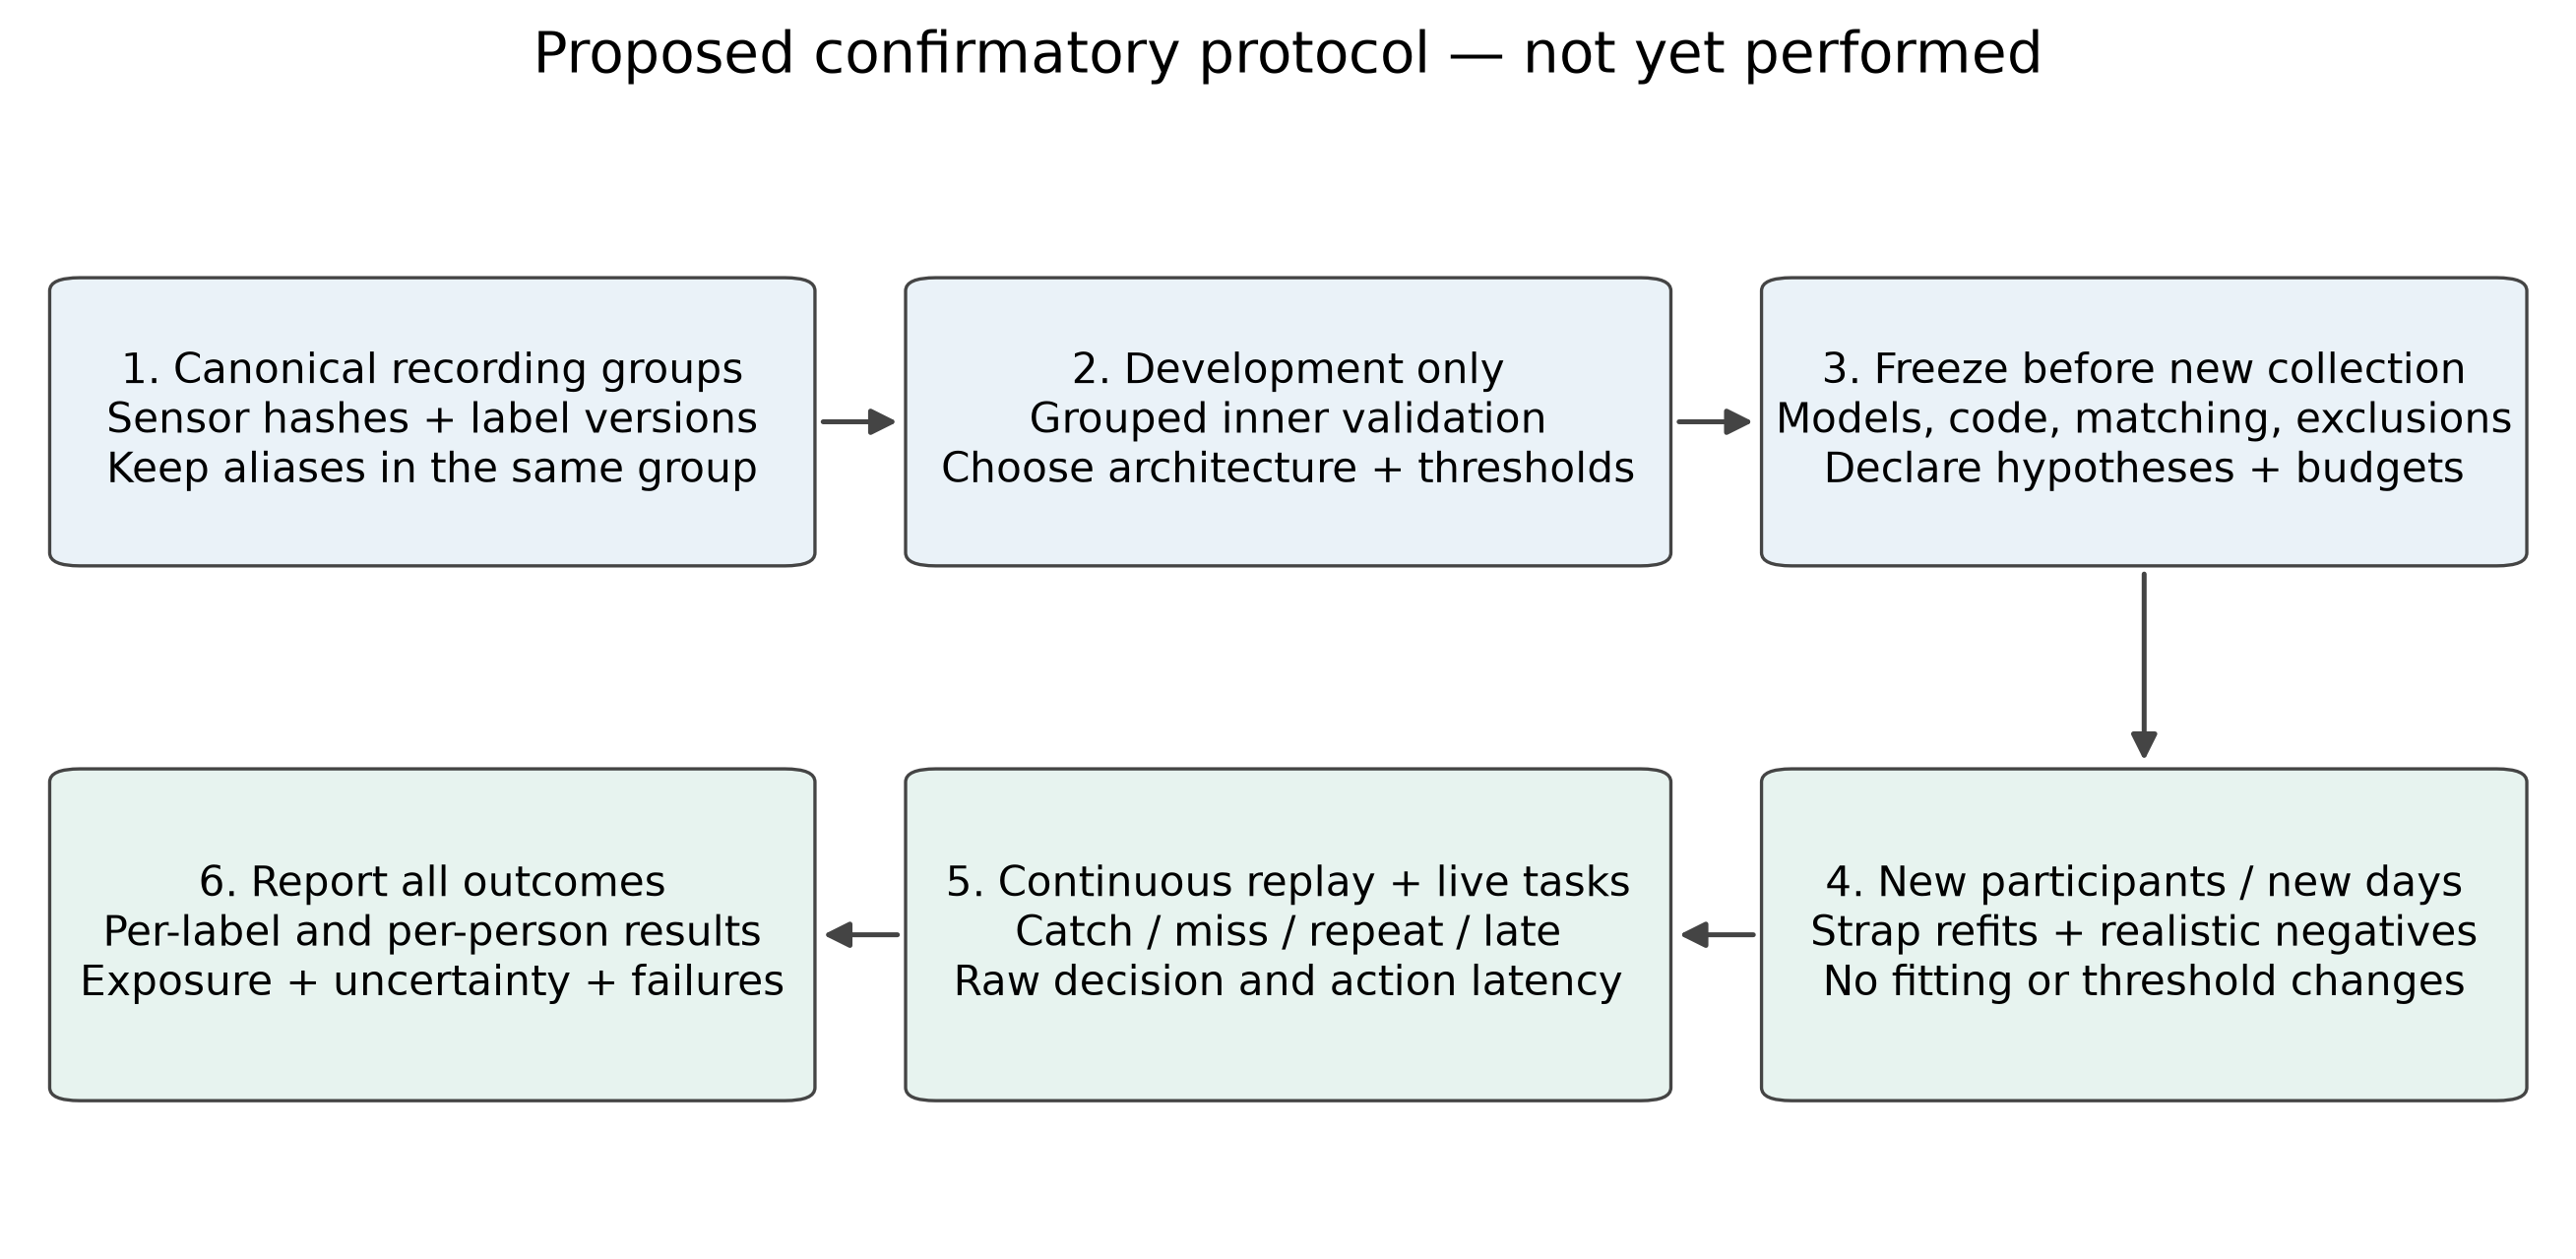
\includegraphics[width=1\linewidth,height=\textheight,keepaspectratio,alt={Proposed development, freeze, prospective collection and continuous/live evaluation sequence.}]{figures/prospective-protocol.png}
\caption{Planned confirmatory workflow: develop, freeze, collect new data, then evaluate continuously and in live use. None of these stages has been carried out yet.}\label{fig-prospective}
\end{widefigure}
\fi

\iffull
\subsect{Matched sensing and preprocessing comparisons}\label{matched-sensing-and-preprocessing-comparisons}
\fi

\iffull
The smallest useful ablation compares IMU-only, PPG-only and fused inputs on the same corrected source groups, then rolling against median scaling, then the CNN against the engineered-feature trees. All variants should share the selection procedure, false-activation target, input rate, exclusions and matching rules. Each may have its own threshold, chosen the same way on development data and never on test data. Synthetic splices are useful, but real pinches after real movement should be tested as well.
\fi

\iffull
\subsect{Personalisation and generalisation}\label{personalisation-and-generalisation}
\fi

\iffull
Different claims need different splits. A personalised claim needs each person's frozen model tested on new days and after the strap is refitted. A user-independent claim needs whole participants held out. Few-shot adaptation needs a calibration block kept separate from the later test. The number of participants and the amount of exposure should be set from pilot variation and the precision we want. New sessions should include ordinary keyboard and mouse use, wrist turns, different arm support and strap fit, and the quiet conditions the interaction assumes. Pinching while the hand moves should be reported separately if it falls outside the intended still-hand use.
\fi

\iffull
\subsect{Interaction and physical fault trials}\label{interaction-and-physical-fault-trials}
\fi

\iffull
A counterbalanced task should compare look--pinch--turn with a conventional volume control, using set practice, target and timeout rules. We would measure completion time, final error, retries, missed grabs and releases, unintended actions, and discomfort and workload. Fault trials should cover stale signals, disconnection and reconnection, the head leaving the target, model replacement and a release while a volume write is still queued. Latency should be broken down into sensing, receipt, scoring, event emission, policy acceptance and the completed output, with clock uncertainty and unavailable intervals reported.
\fi

\iffull
\subsect{Testing in a headset}\label{testing-in-a-headset}
\fi

\iffull
A natural next step is to repeat the selection task inside an AR or VR headset, using the headset's own head or eye tracking for targeting and the watch for pinch-in and pinch-out. Useful comparisons would be the headset's built-in camera pinch alone, the watch pinch alone, and both combined, including trials with the hand deliberately kept out of the cameras' view. The same event-level measures (recall, false activations per hour of no-gesture time, latency) would let the results be compared directly with the desktop study.

\fi
% Shared section: used by paper-ieee.tex, paper-lncs.tex and report.tex.
% Use \sect / \subsect for headings (see README), never \section directly.

\sect{Conclusion}\label{conclusion}

\iffull
Consumer head tracking and smartwatch optical and inertial sensing can be combined into a working desktop interaction, with explicit grab, release and cancellation. Our audit shows what the current data support. The 37 hand-labelled exports reduce to 28 distinct streams, the pinch-in model's training and evaluation sets share no stream, and its result of 47 of 57 starts caught with no false activations in 0.48\,h can be reproduced, but it is development evidence rather than an independent test. Historical camera-label results varied widely from day to day, which a single pooled number hides. The next step is not a bigger model. It is matched comparisons of label versions and sensing modalities, followed by a frozen prospective study with real interaction tasks.

\else
Consumer head tracking and smartwatch PPG and inertial sensing can be combined into a working hands-free interaction with explicit grab, release and cancellation. On one participant's held-out recordings, the pinch-in detector caught 47 of 57 starts with no false activations in 0.48\,h, a reproducible development result rather than an independent test. The next steps are matched modality comparisons, a frozen multi-participant study with real tasks, and trials inside AR/VR headsets.
\fi

\bibliographystyle{plainnat}
\bibliography{refs}

\appendix
% Report-only appendices.
\chapter{Dataset Inventory}
\todo{Recording inventory and hashes. Source: docs/paper/revision-assets/hand-labelled-inventory.csv.}

\chapter{User Guide}
\todo{How to run the system. Source: docs/using-the-application.md.}

\end{document}
